% Hamad Medical Corporation
% Georges Younes

\section{Model Generation}\label{sec:generation_3d}

\subsection{Generation of Surface Models}\label{ssec:generation_surface}

We have designed five geometric models of the surgical tooltips (\autoref{fig:endowrist_generation}) based on the EndoWrist instruments of the da Vinci Xi surgical robot. These models were selected based on the five basic interactions of the surgical tooltip with the anatomical structures, which include the following:
\begin{enumerate}
  \item Cauterization of the tissue,
  \item Stitching using needles,
  \item Applying clips on vascular structures,
  \item Cutting using scissors, and
  \item Grasping of the tissues.
\end{enumerate}

\begin{figure}
  \centering%
  \subbottom[Cautery]{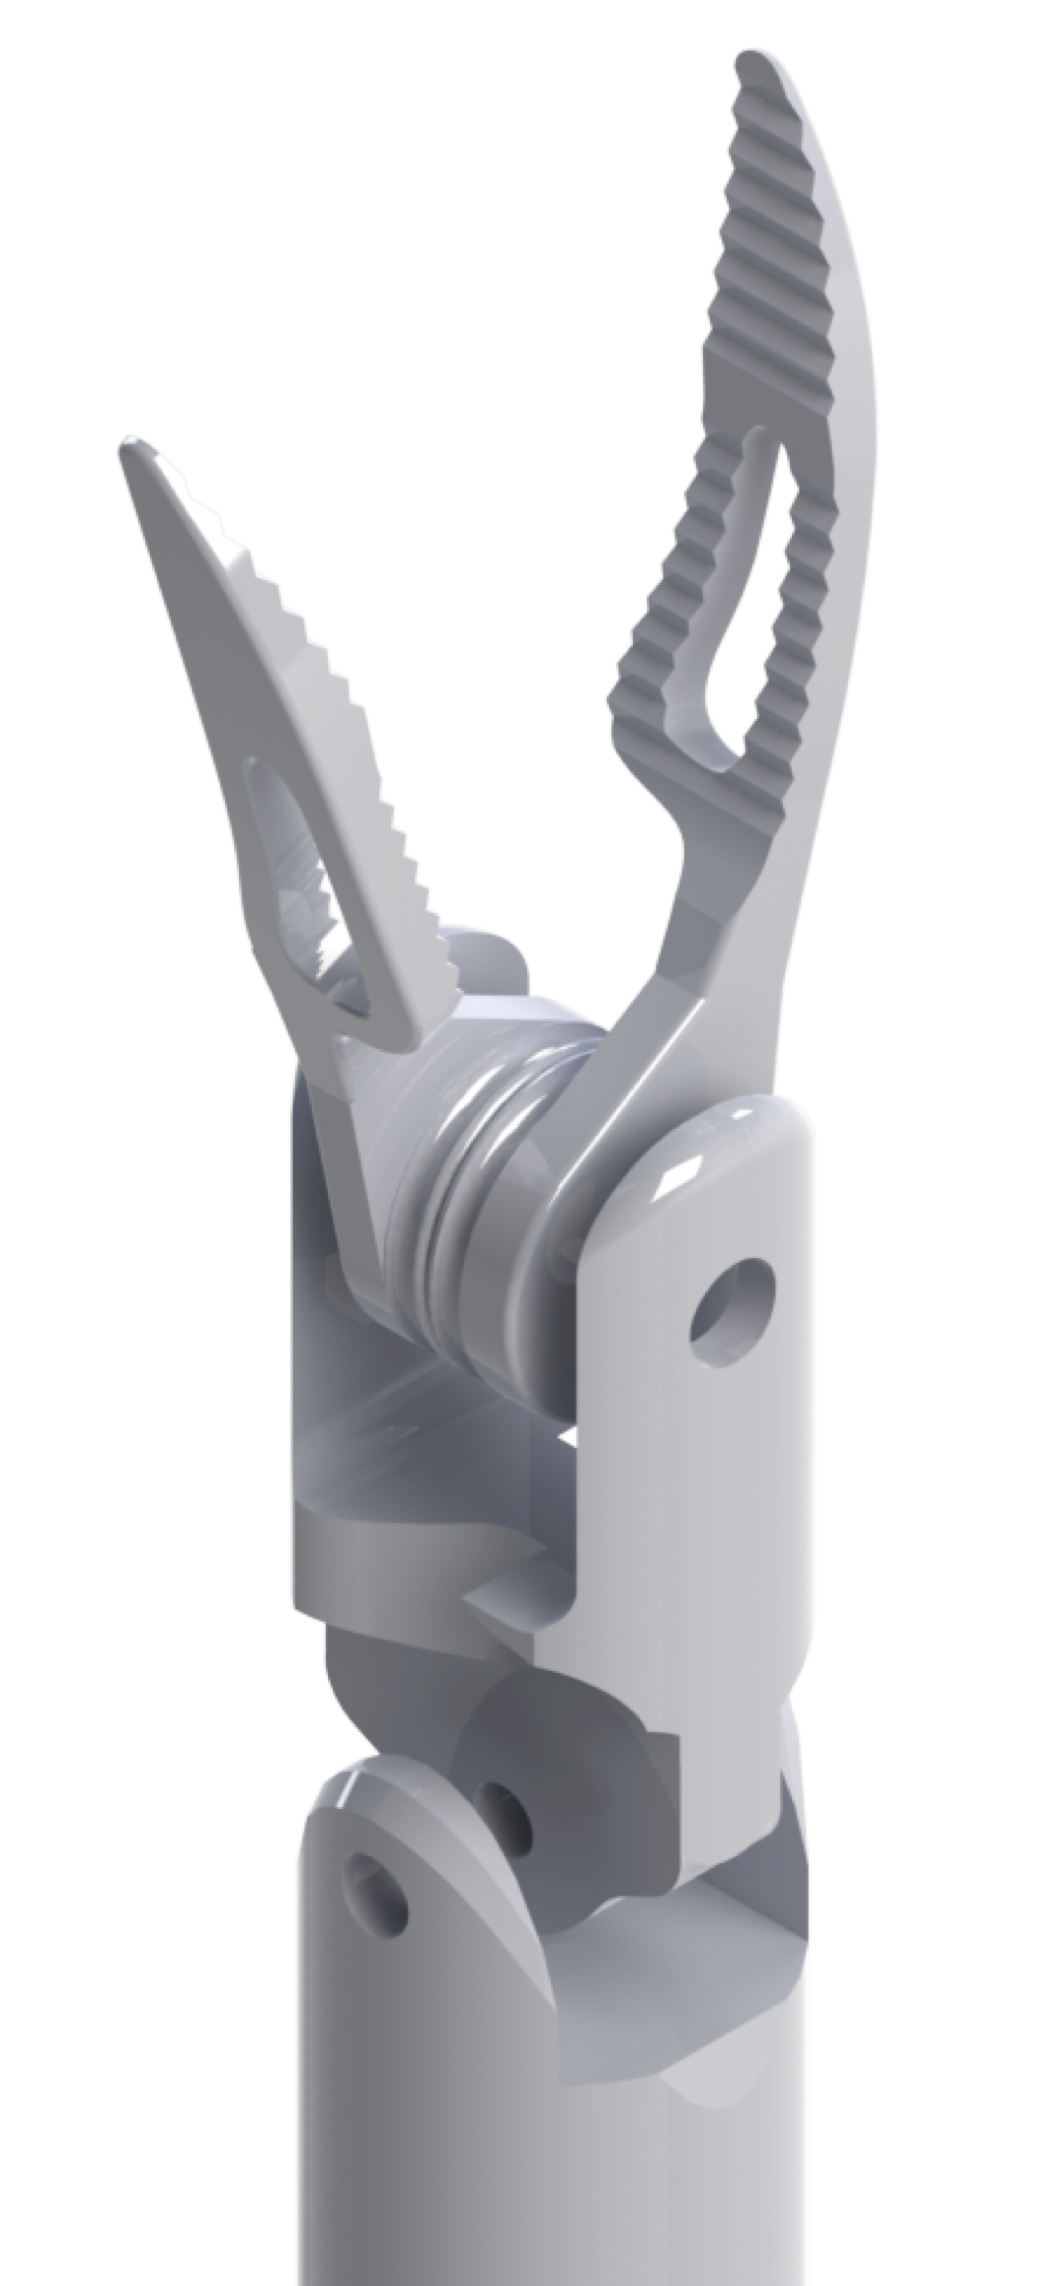
\includegraphics[width=0.22\textwidth]{models/endowirst_cautery}}
  \subbottom[Needle driver]{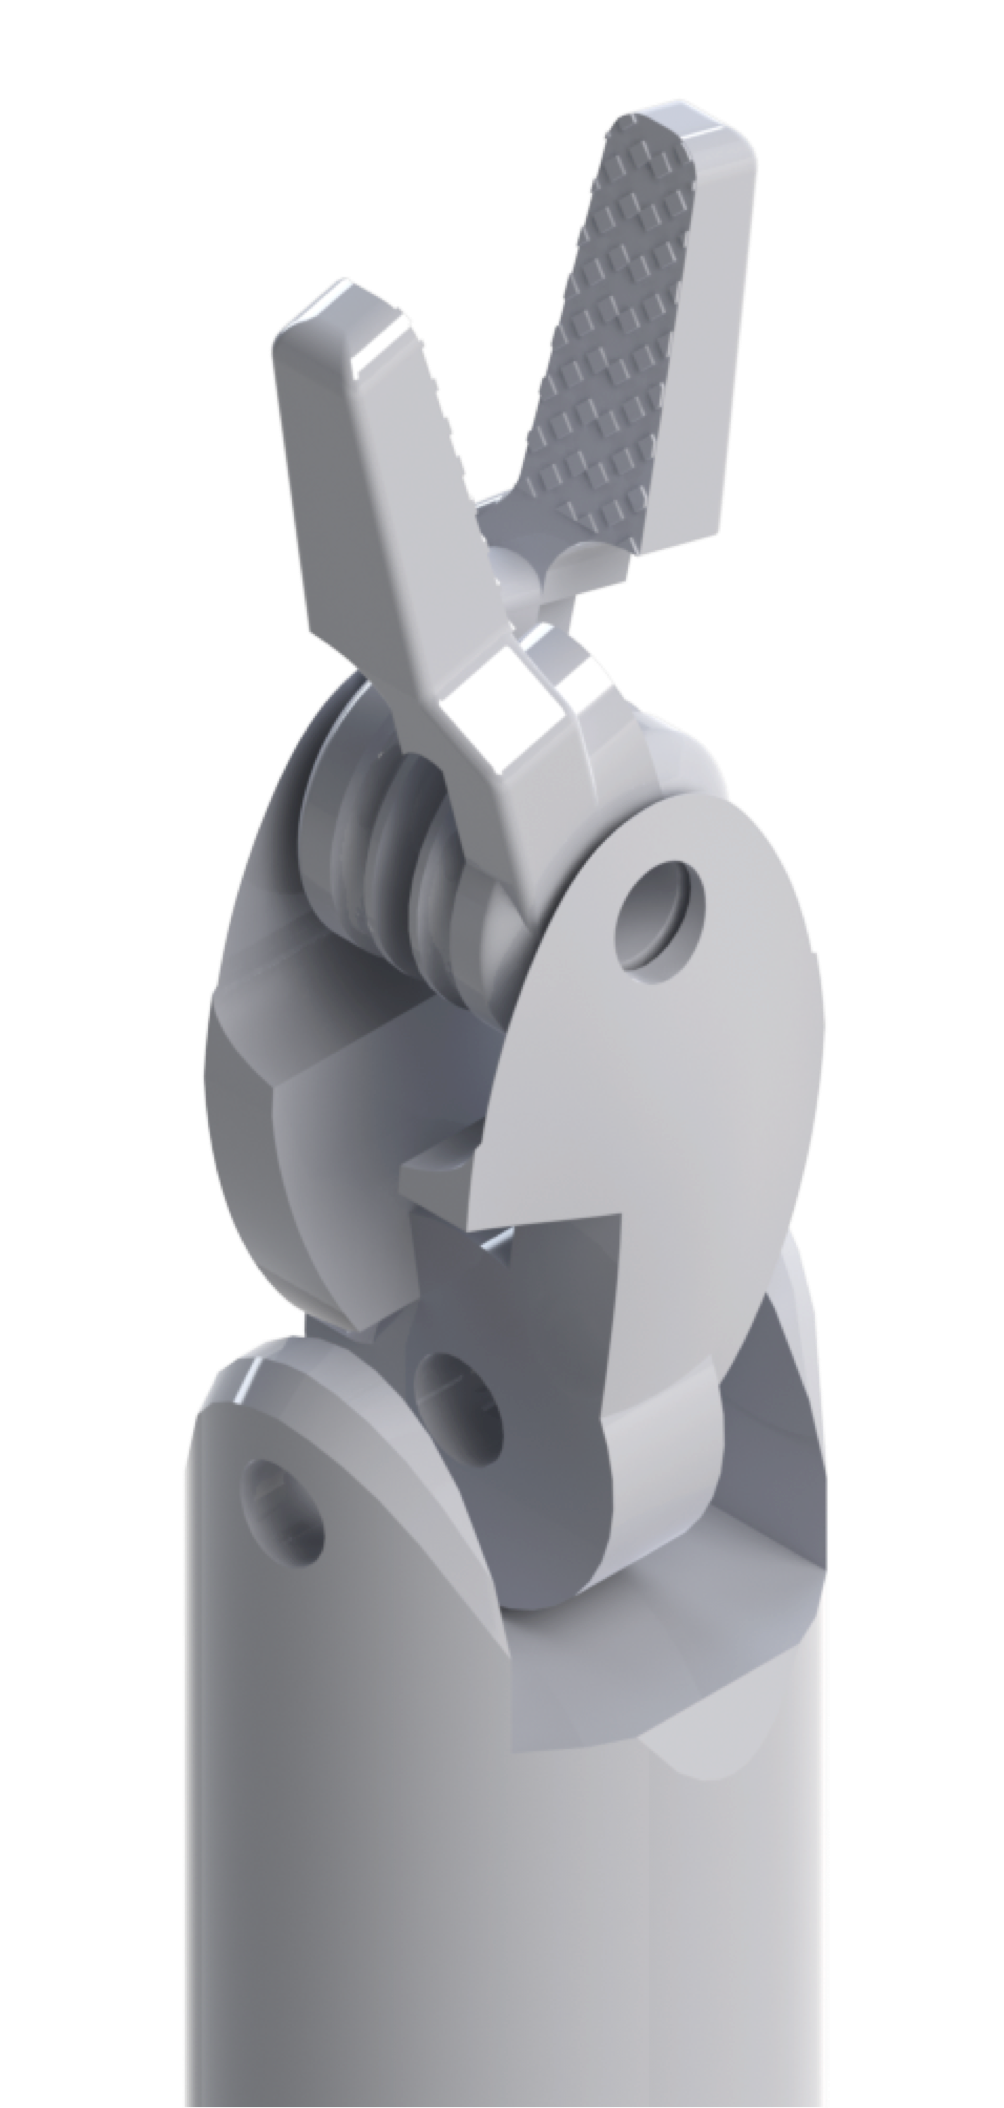
\includegraphics[width=0.17\linewidth]{models/endowirst_driver}}
  \subbottom[Clip applier]{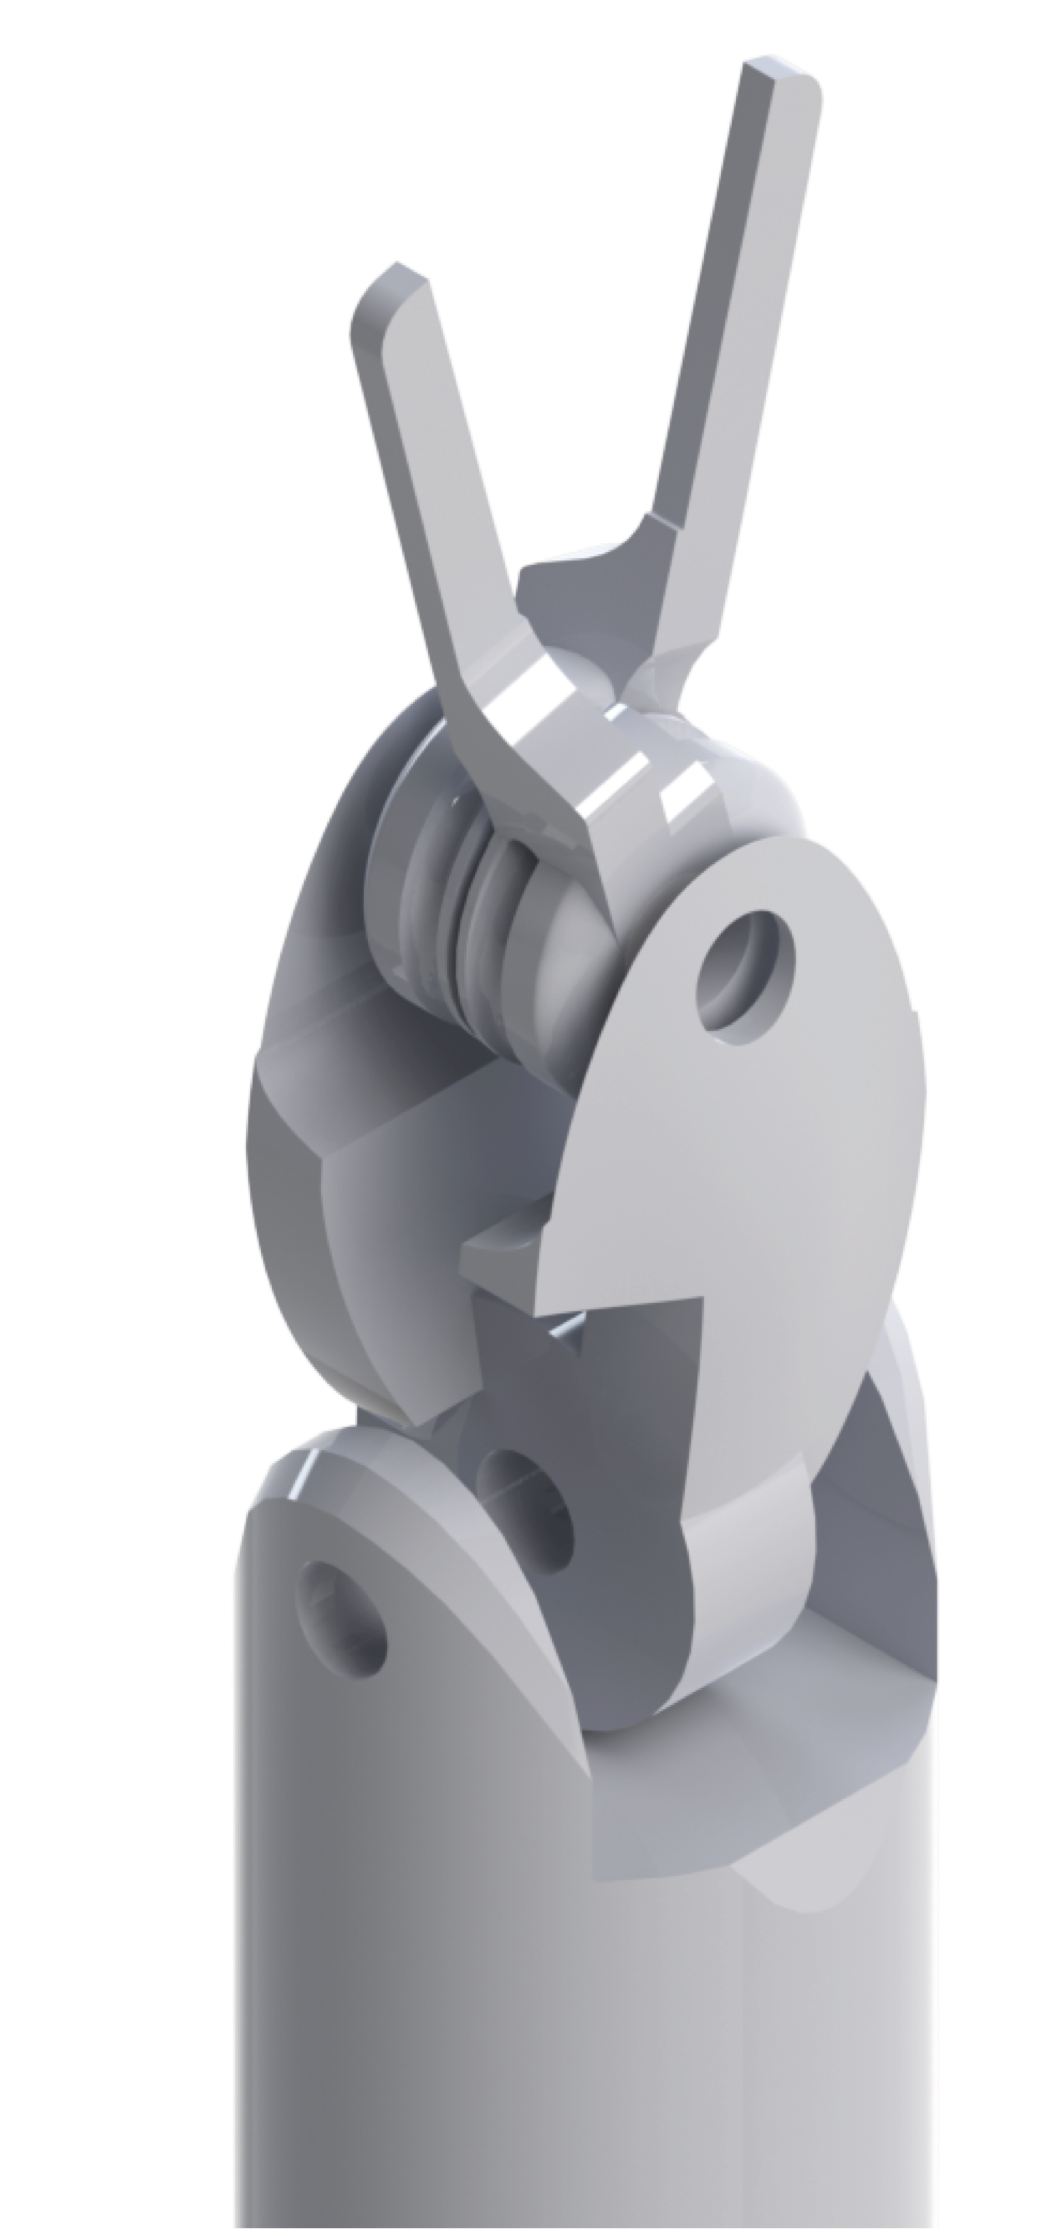
\includegraphics[width=0.17\linewidth]{models/endowirst_clip}}
  \subbottom[Scissors]{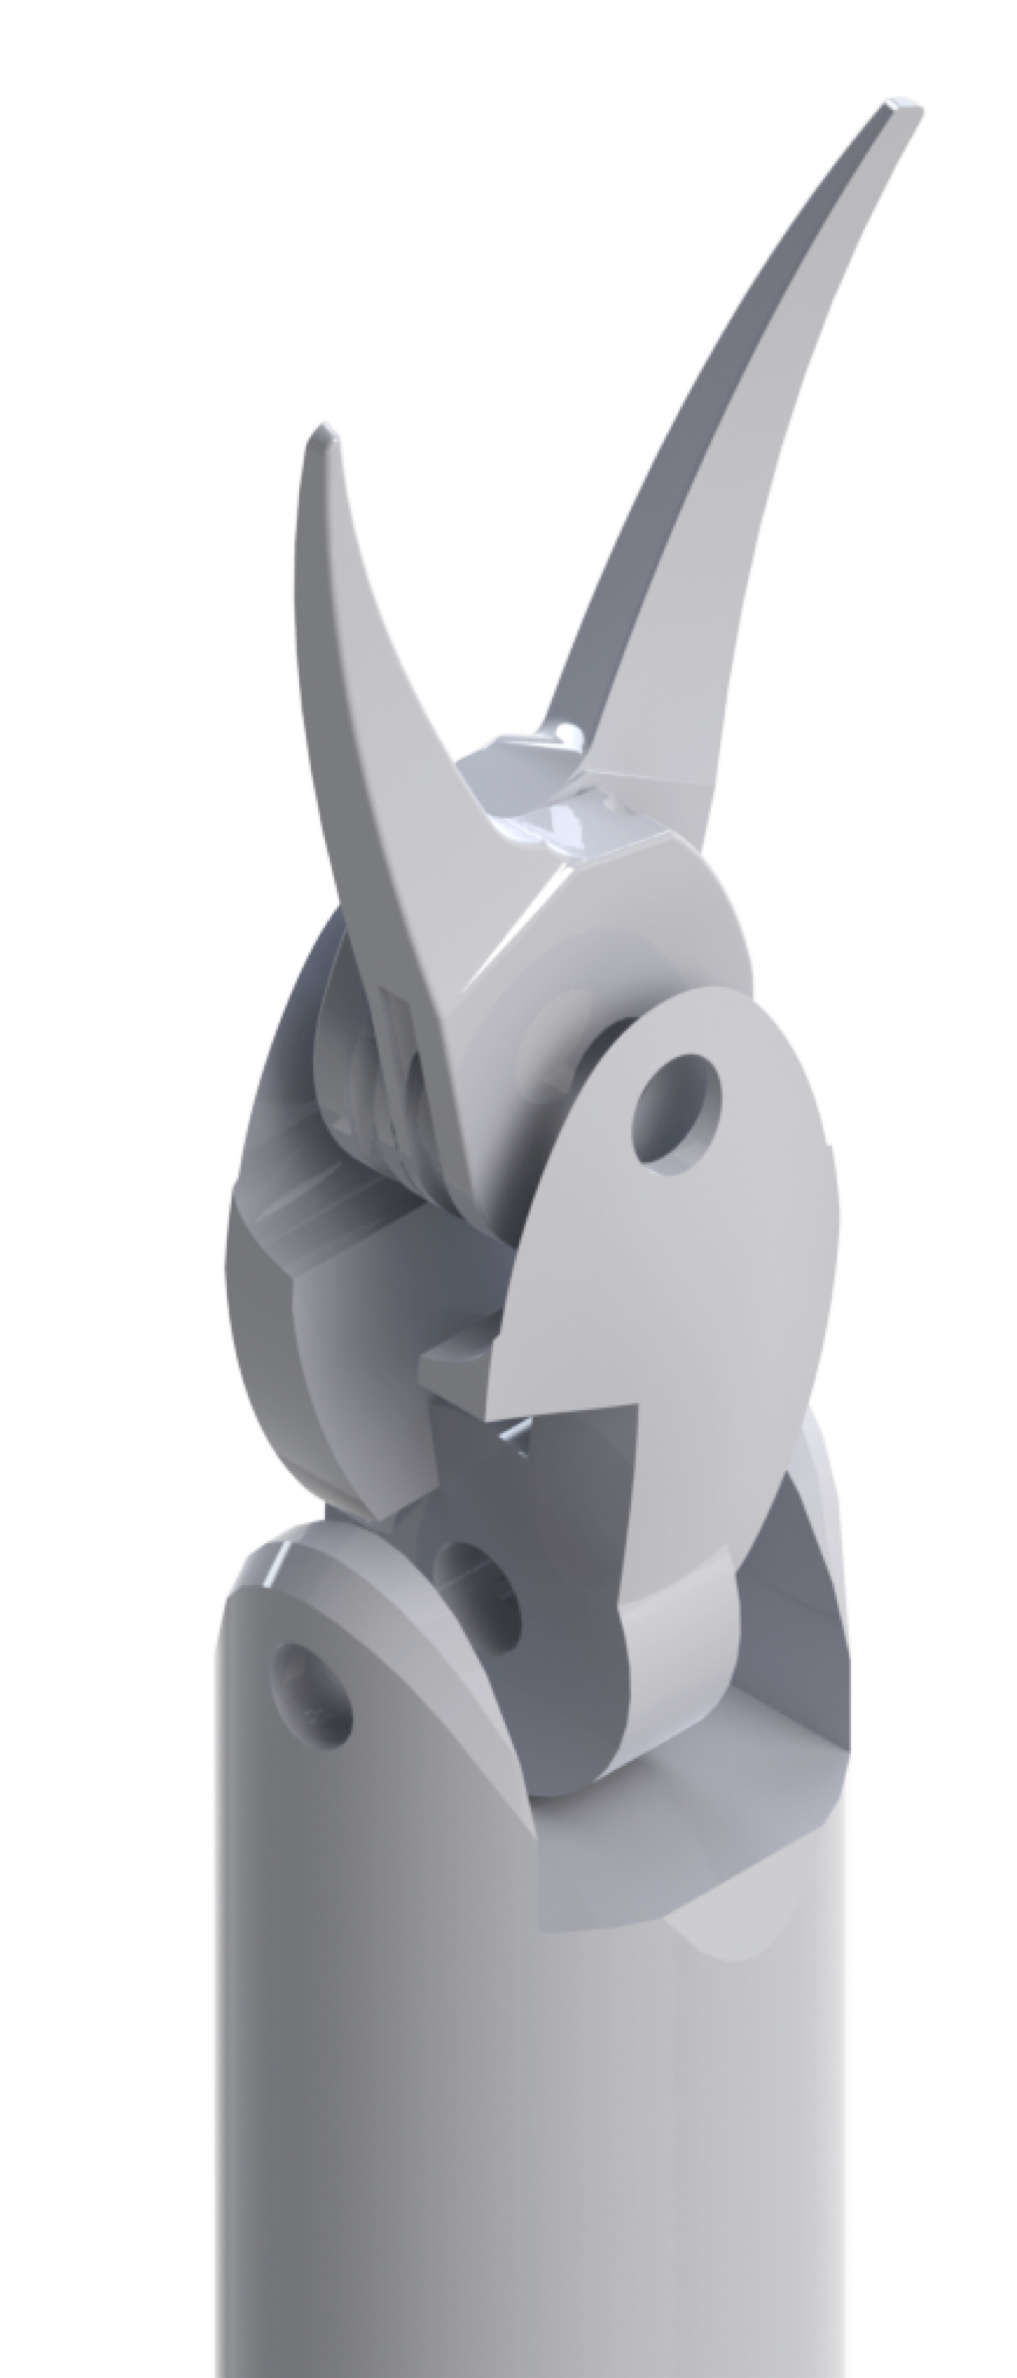
\includegraphics[width=0.17\linewidth]{models/endowirst_scissor}}
  \subbottom[Graspers]{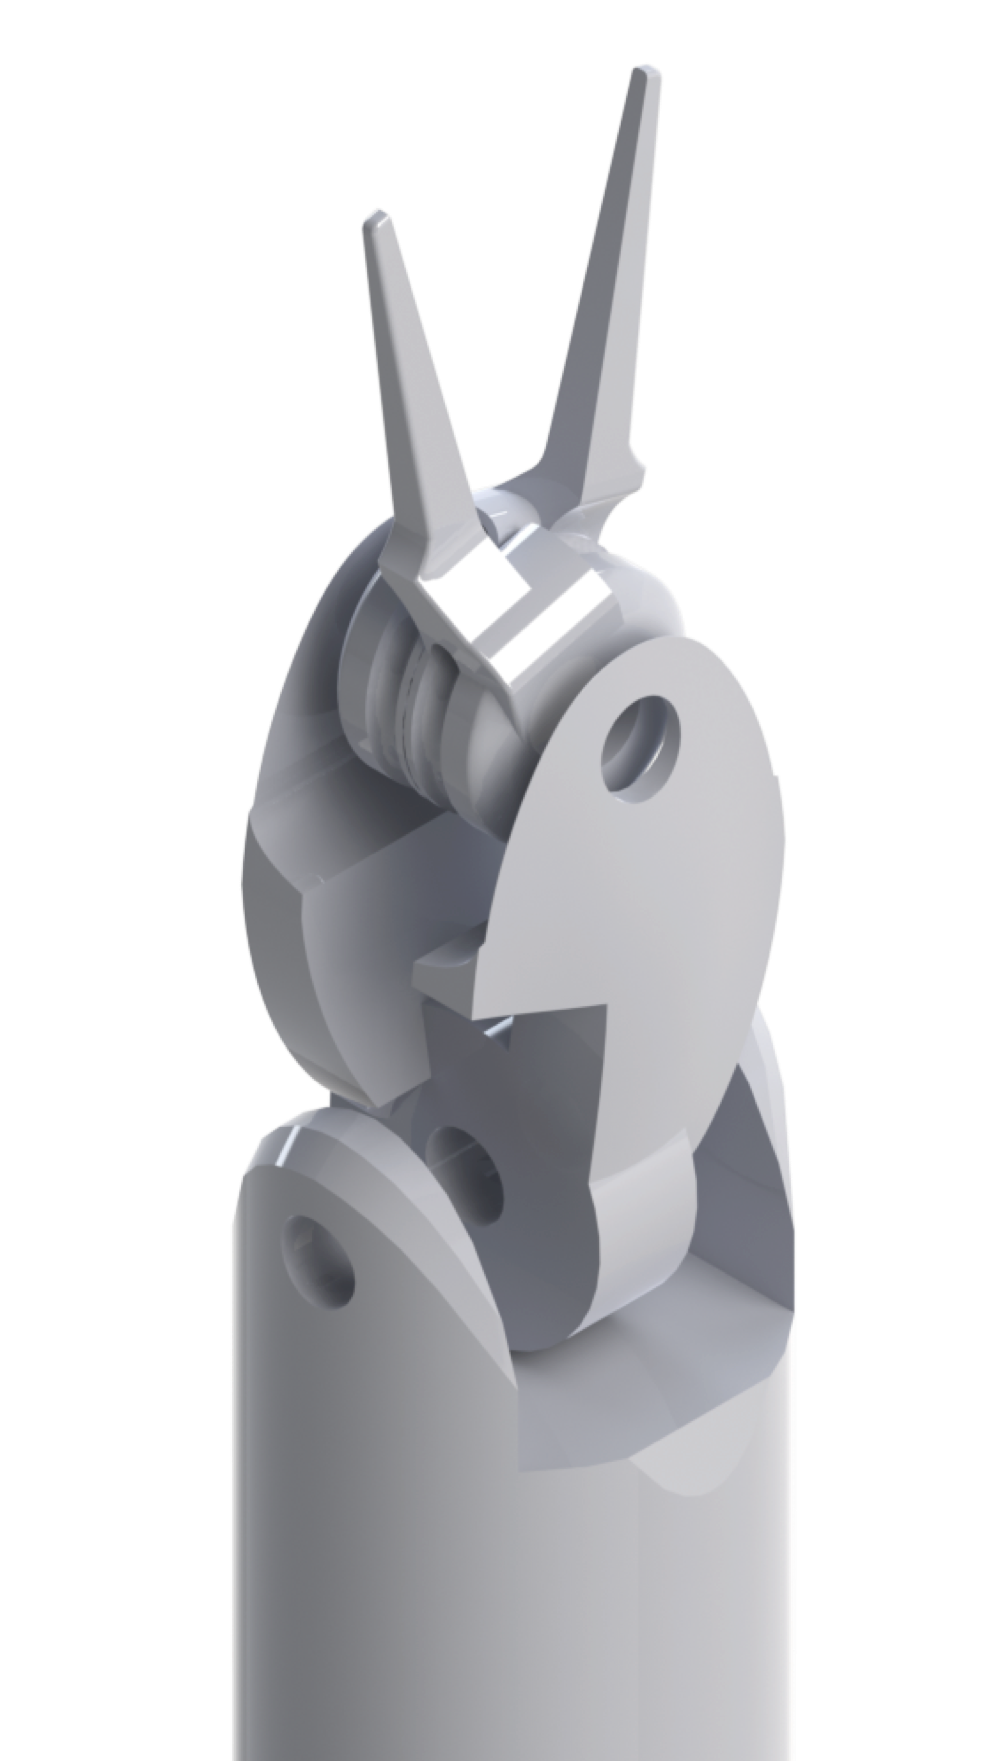
\includegraphics[width=0.20\linewidth]{models/endowirst_grasper}}
  \caption{Snapshots of EndoWrist \acr{3d} \acr{cad} models}\label{fig:endowrist_generation}
\end{figure}

Shapes of the link and inter-link distances of the EndoWrist instrument were measured in detail. \acr{3d} virtual models were then recreated using SolidWorks, a \acr{cad} toolset, and are visualized in \autoref{fig:endowrist_generation}.

\begin{figure}
  \centering%
  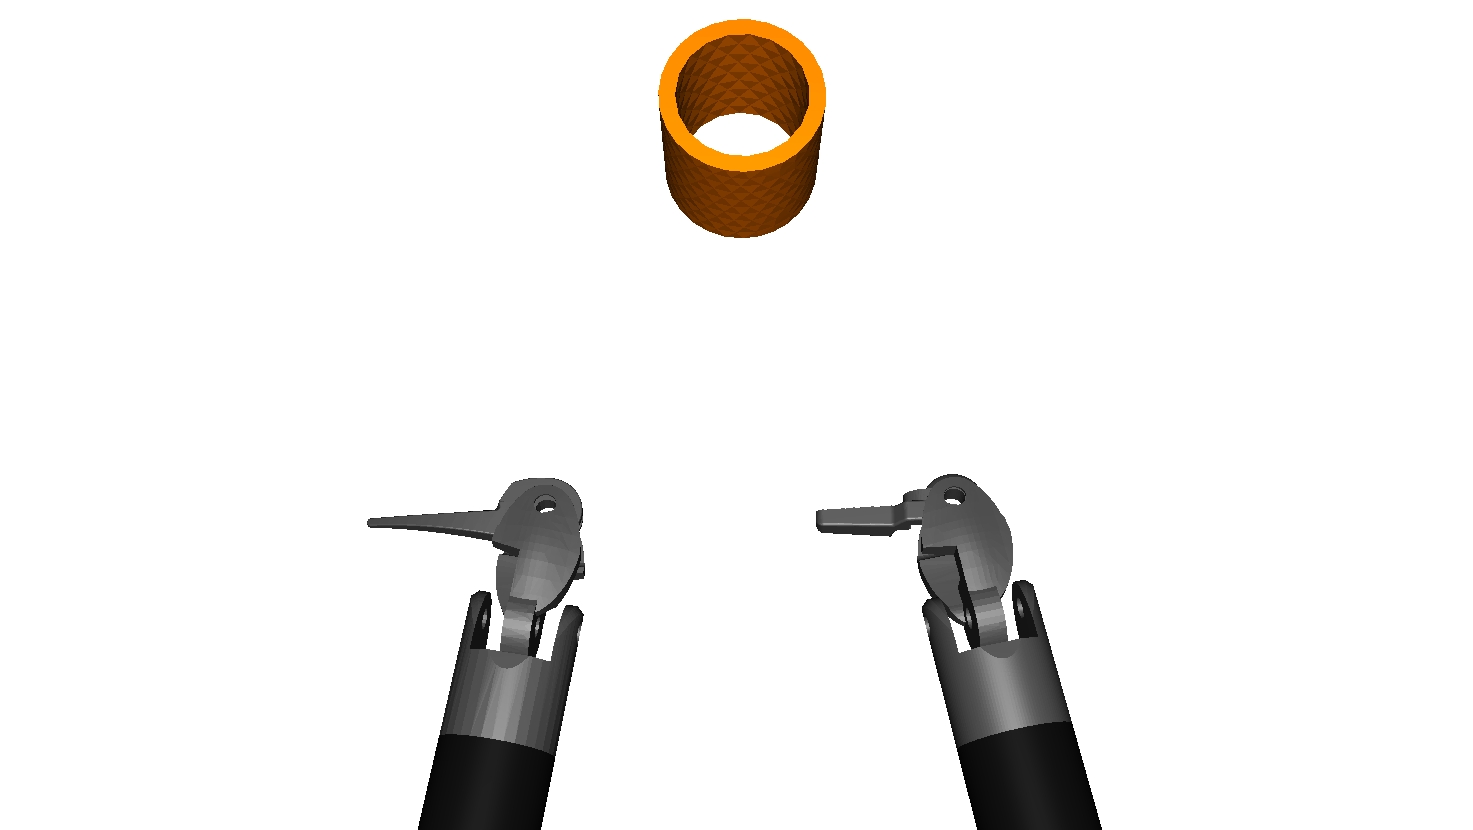
\includegraphics[width=\linewidth,frame]{models/decimated}
  \caption{Decimated model of an EndoWrist instrument (left) \vs original model (right). The decimated models are used to accelerate the collision detection and response}\label{fig:decimated}
\end{figure}

We identified \acr{ut} in \acr{rarp} performed with the da Vinci surgical Xi robot (\acr{isi}) as the clinical procedure to be simulated on the surgical simulator being developed. The critical steps of the \acr{rarp} procedure were analyzed and for each step, organs/tissues involved during the procedure were delineated on anonymized \acr{mri} images of the pelvic region. From delineated data, \acr{3d} surface meshes of the organ were generated.

The main organ models, a total of 19, included: prostate, rectum, seminal vesicle, urinary bladder, femoral vein, artery and nerve, femur neck, sacrum coccyx, bilateral coccygeus, levator-ani and obturator-internus muscles, the prostatic pedicles and neurovascular bundle, and perirectal fat.

\begin{figure}
  \centering%
  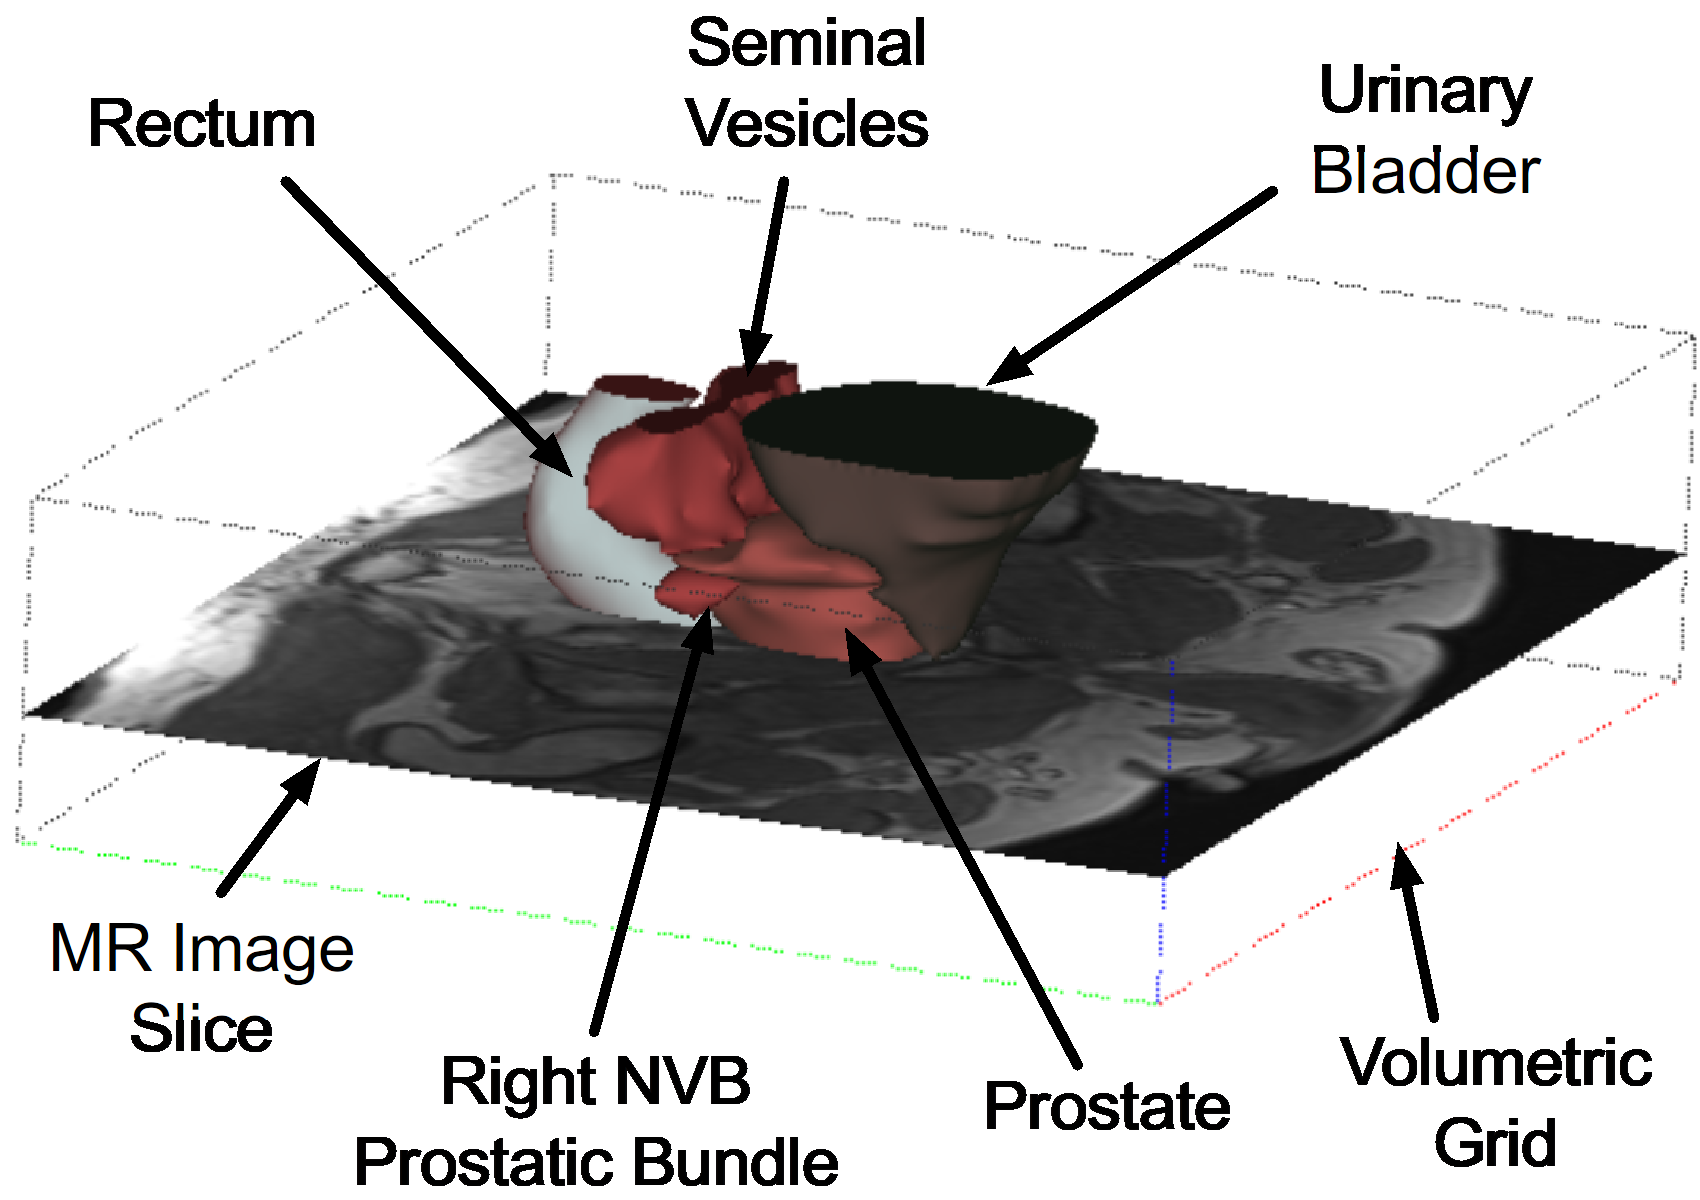
\includegraphics[width=0.6\linewidth]{models/augmented_pelvic}
  \caption{Snapshot of organ models generated from \acr{mri} images}\label{fig:organ_generation}
\end{figure}

We used CAD packages to generate surface models of the required organs and surrounding tissue, as shown in succession below: The urethra, the prostate, and surrounding tissue.

\begin{figure}
  \centering%
  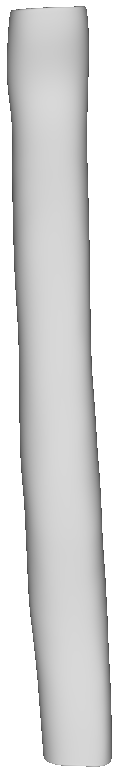
\includegraphics[height=22ex]{models/surface_u_crop}\hfill%
  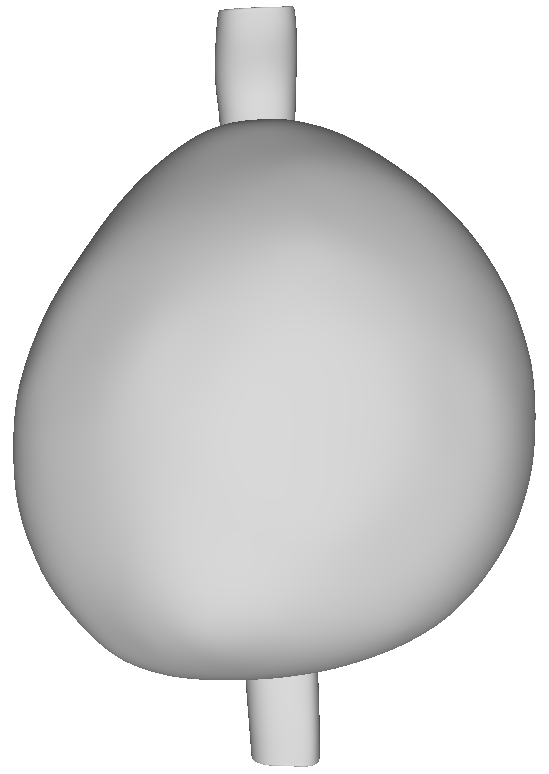
\includegraphics[height=22ex]{models/surface_up_crop}\hfill%
  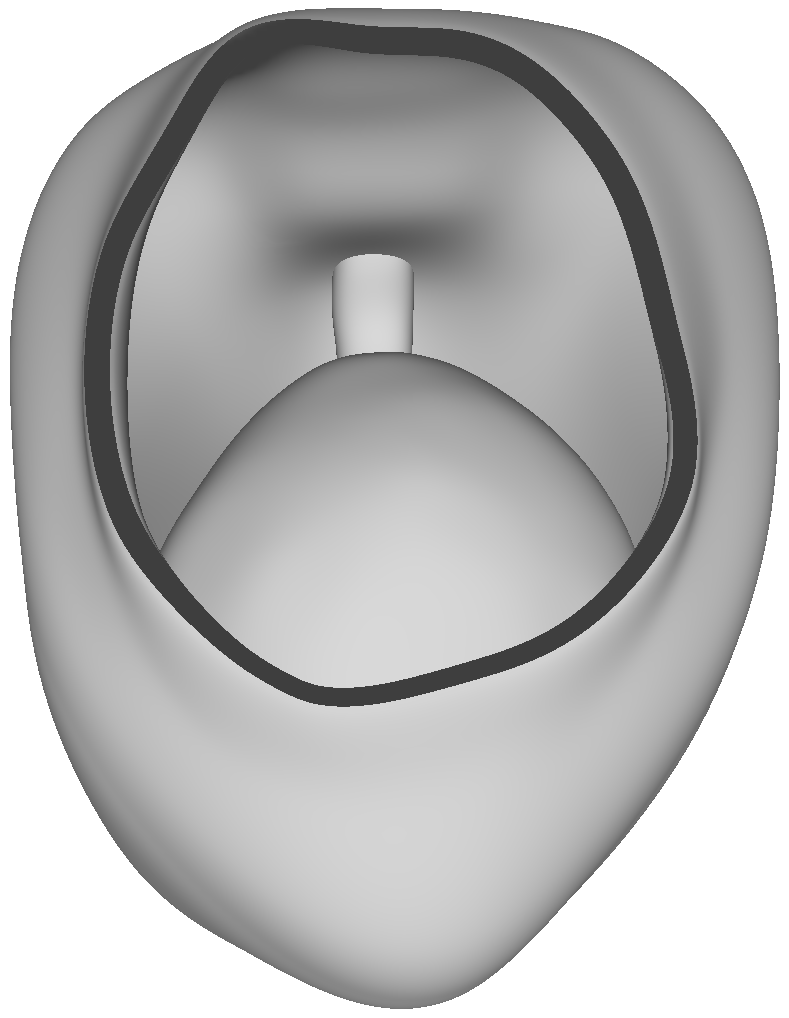
\includegraphics[height=22ex]{models/surface_upb_crop}\hfill%
  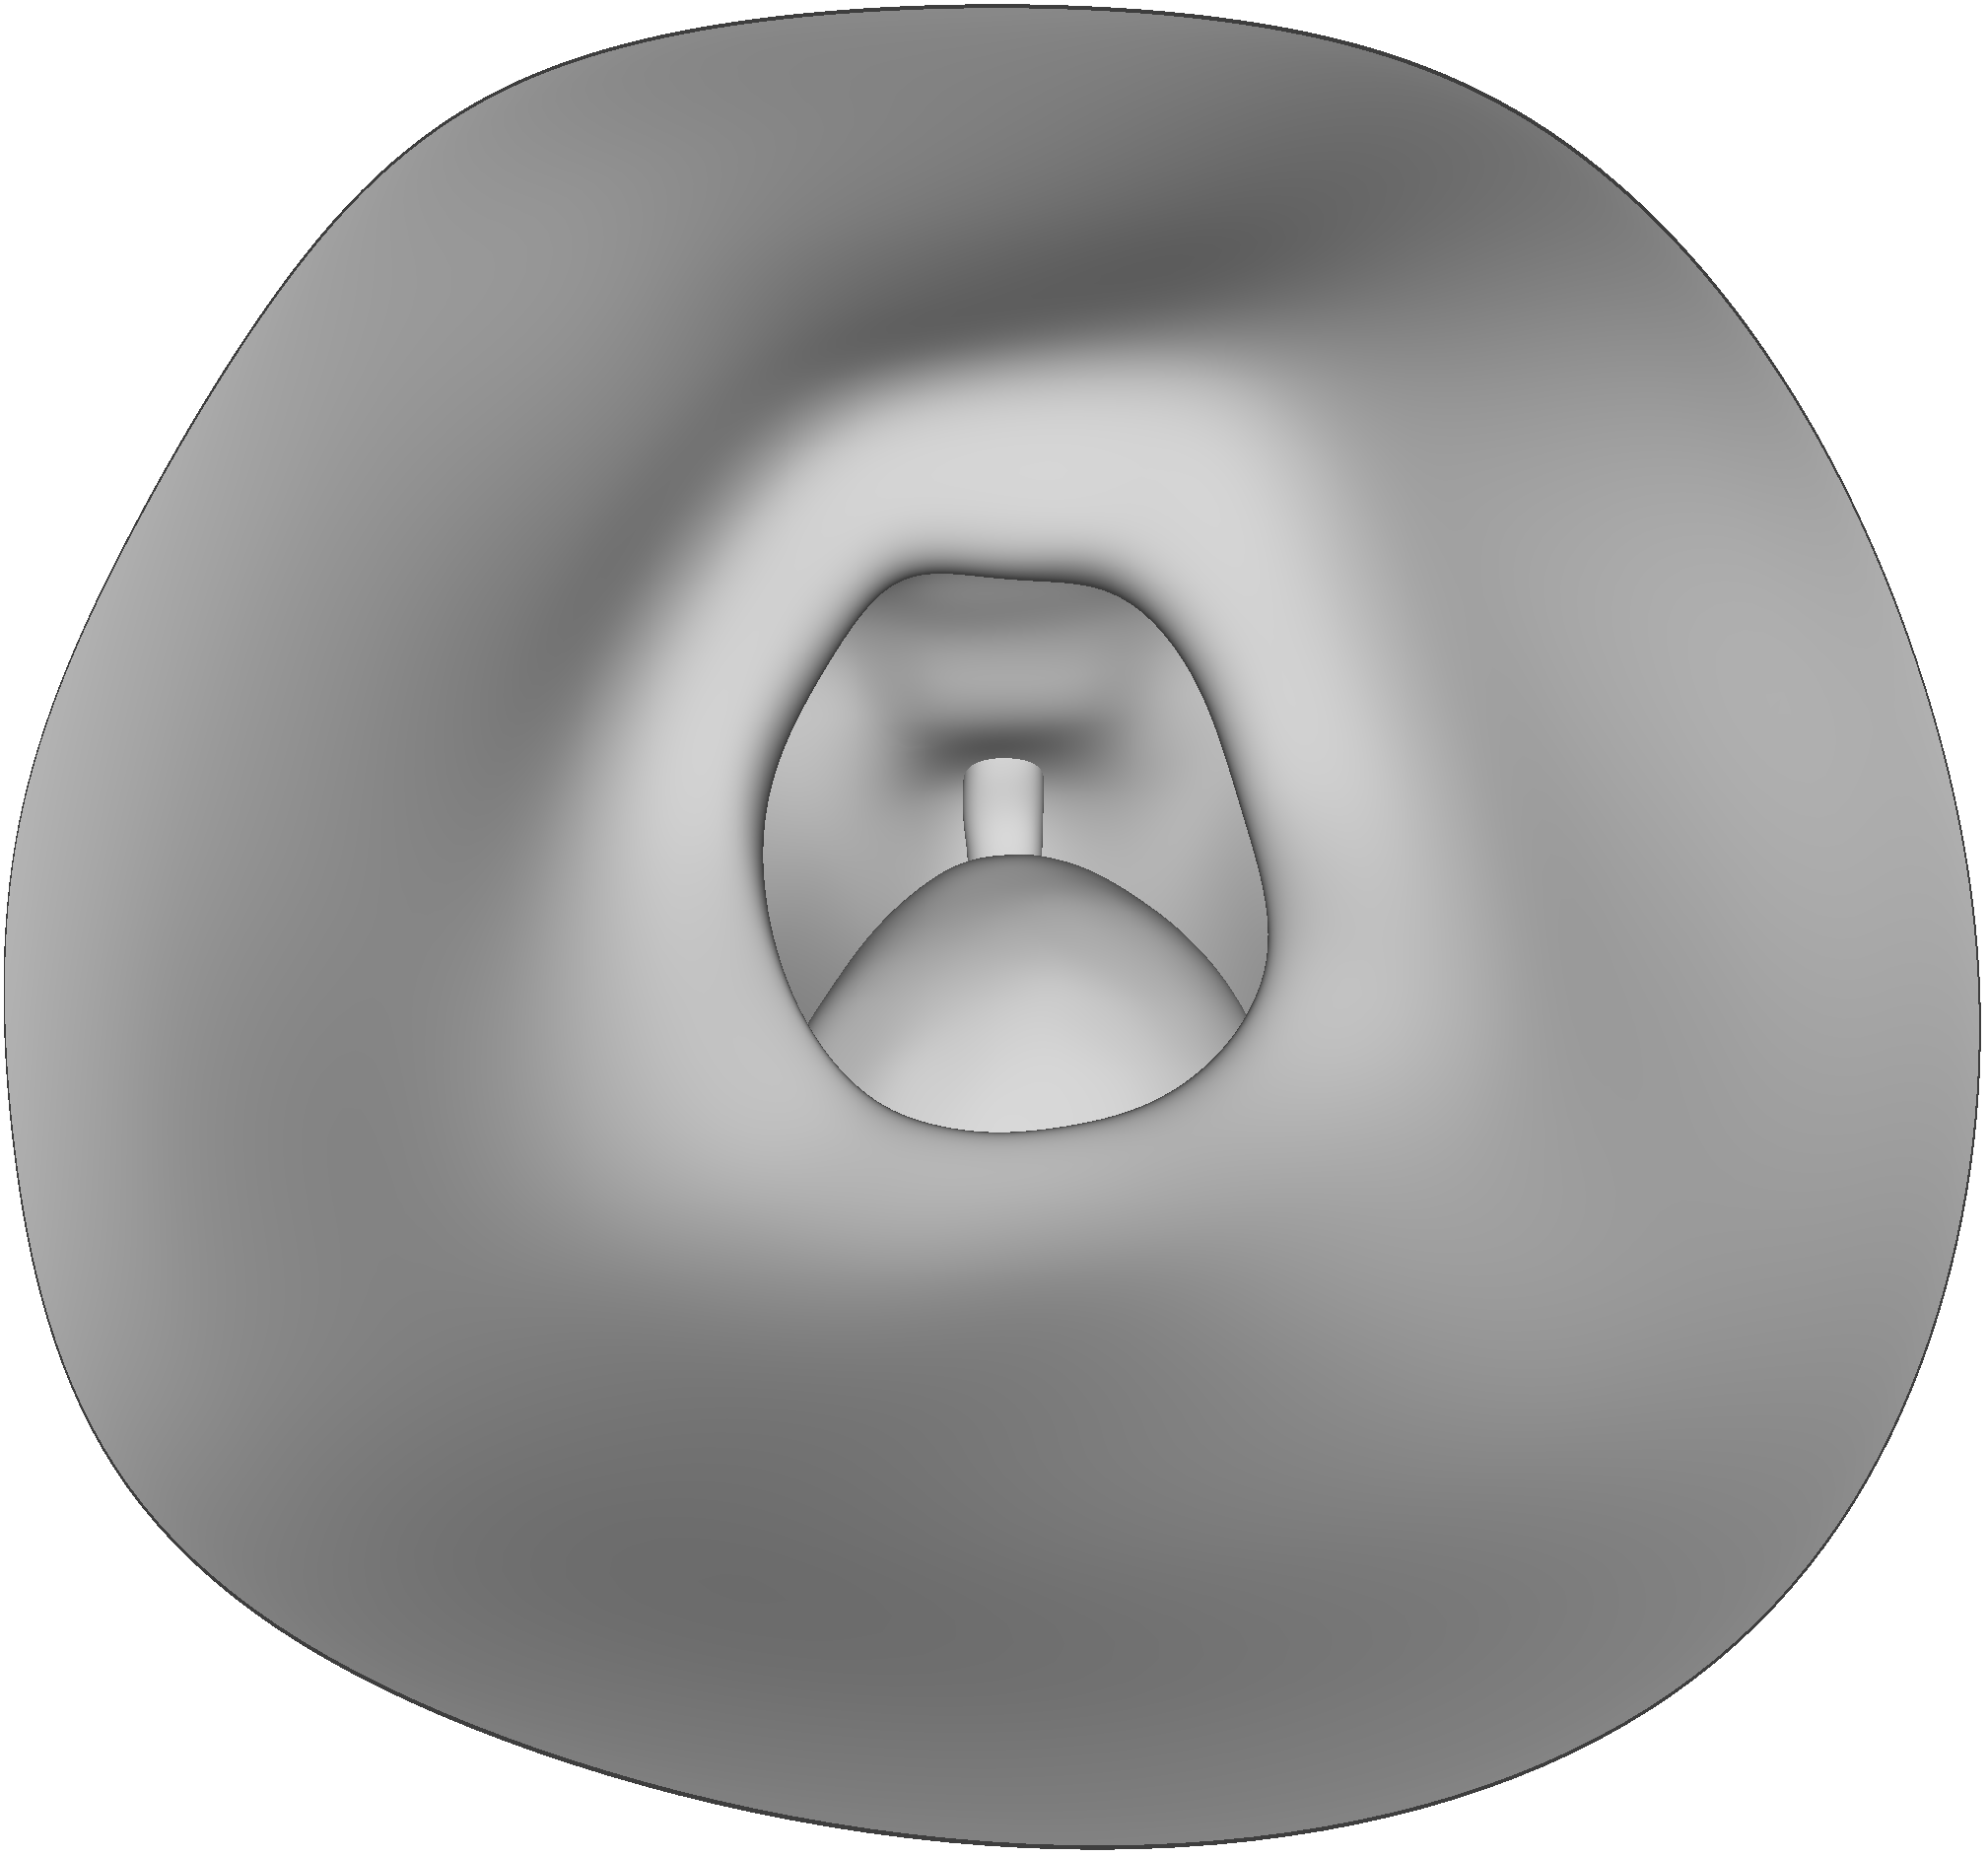
\includegraphics[height=22ex]{models/surface_upbt_crop}
  \caption{---}\label{fig:surface_meshes}
\end{figure}

We've generated meshes from MRI scans of a phantom as shown in \autoref{fig:pelvic_osirix} and \autoref{fig:pelvic_models}.

\begin{figure}
  \centering%
	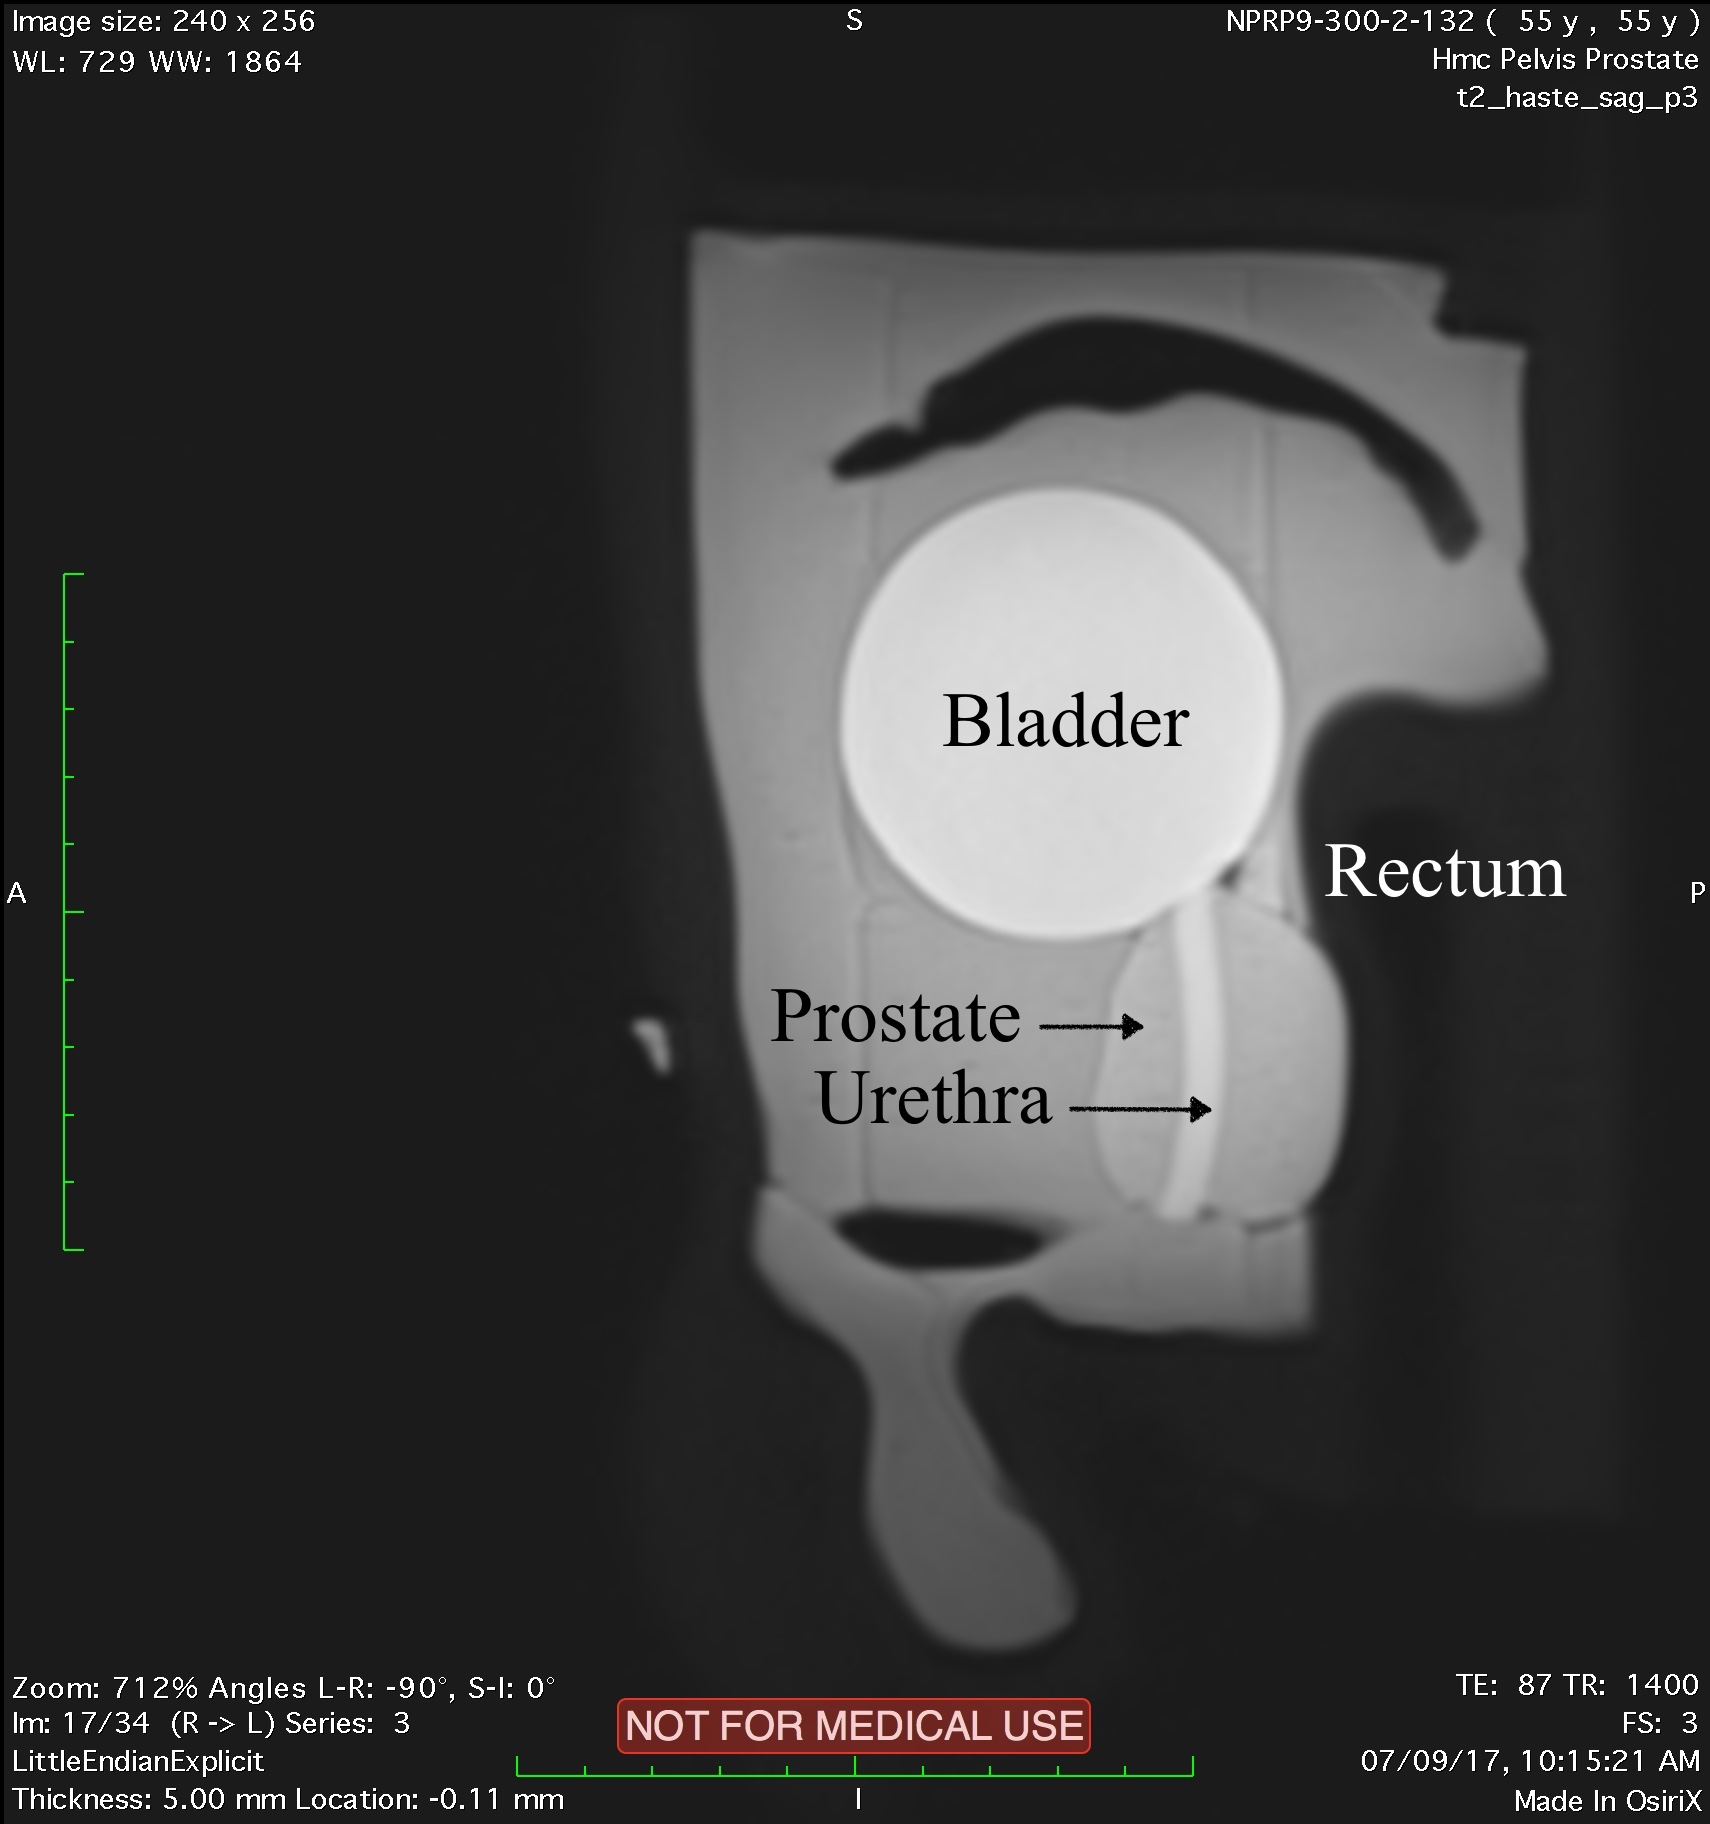
\includegraphics[width=0.5\linewidth]{models/pelvic_mri}\\[10ex]
	\caption{Pelvic \acr{mri} image}\label{fig:pelvic_osirix}
\end{figure}
\begin{figure}
  \centering%
	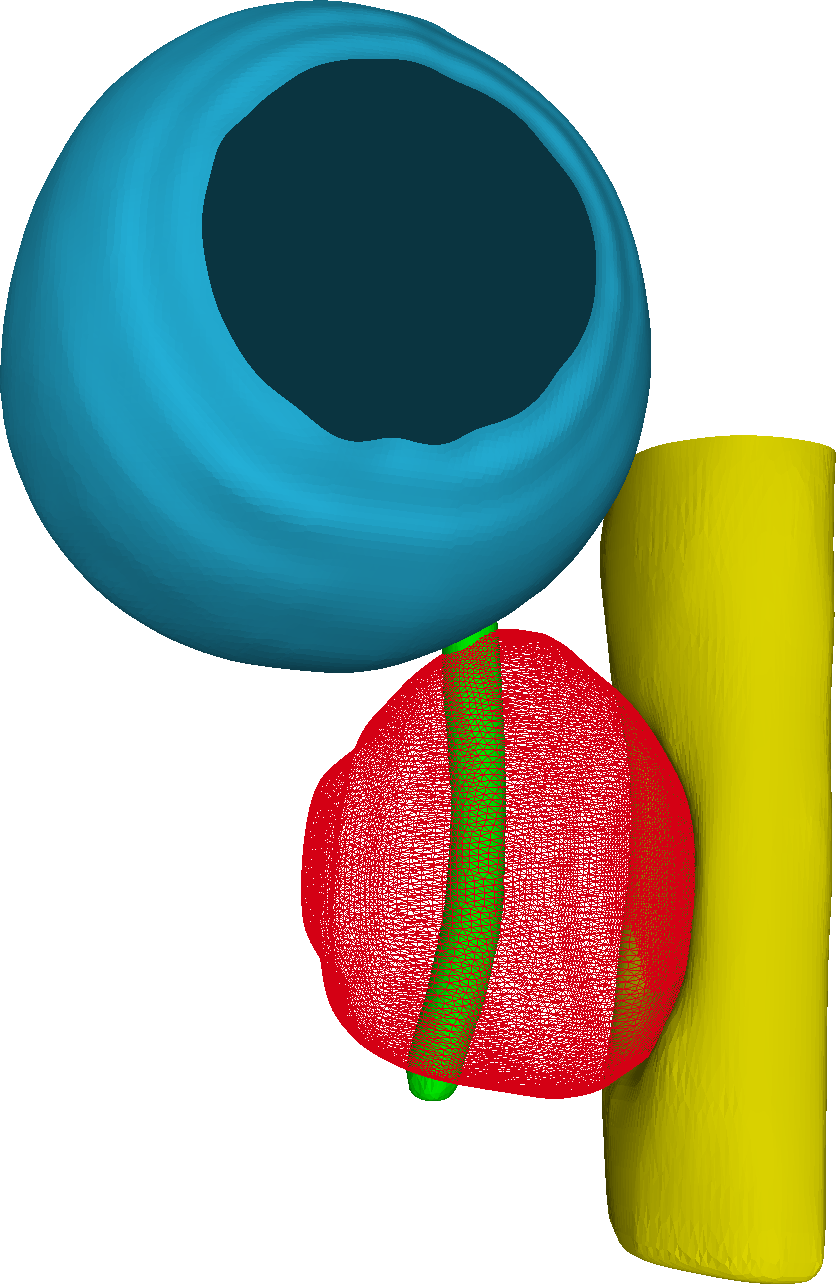
\includegraphics[width=0.25\linewidth]{models/pelvic_model_view_1}\hfill%
	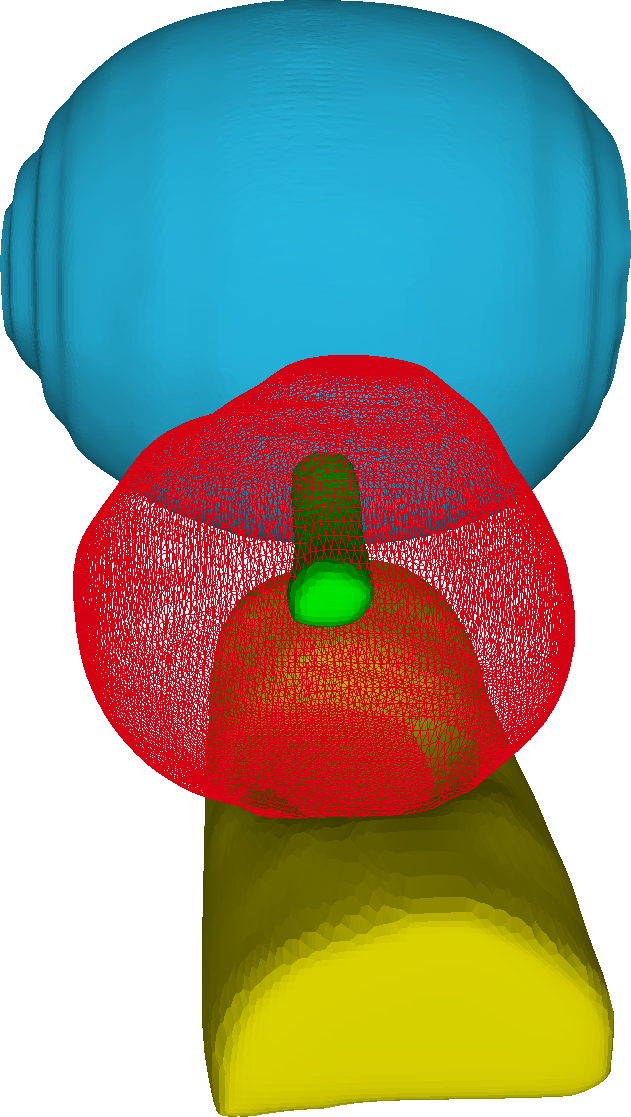
\includegraphics[width=0.20\linewidth]{models/pelvic_model_view_2}\hfill%
	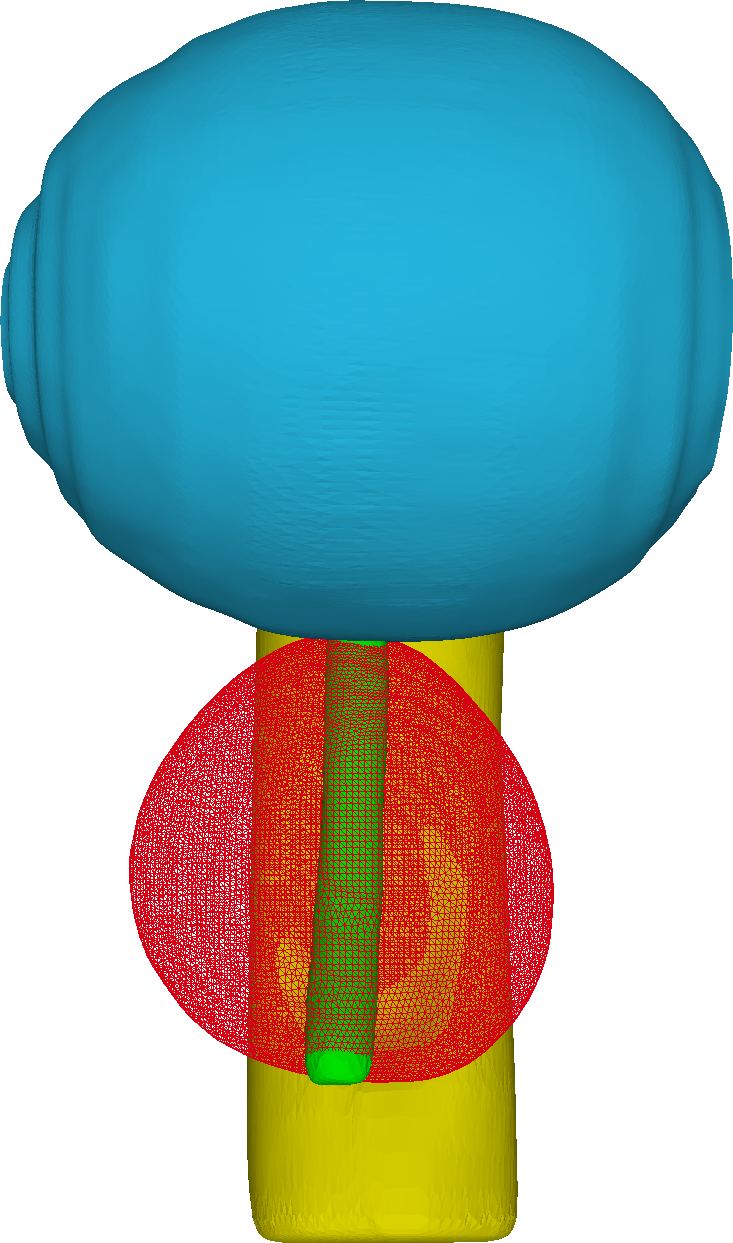
\includegraphics[width=0.20\linewidth]{models/pelvic_model_view_3}
	\caption{Pelvic surfaces generated from an \acr{mri} image}\label{fig:pelvic_models}
\end{figure}

\begin{figure}
  \centering%
  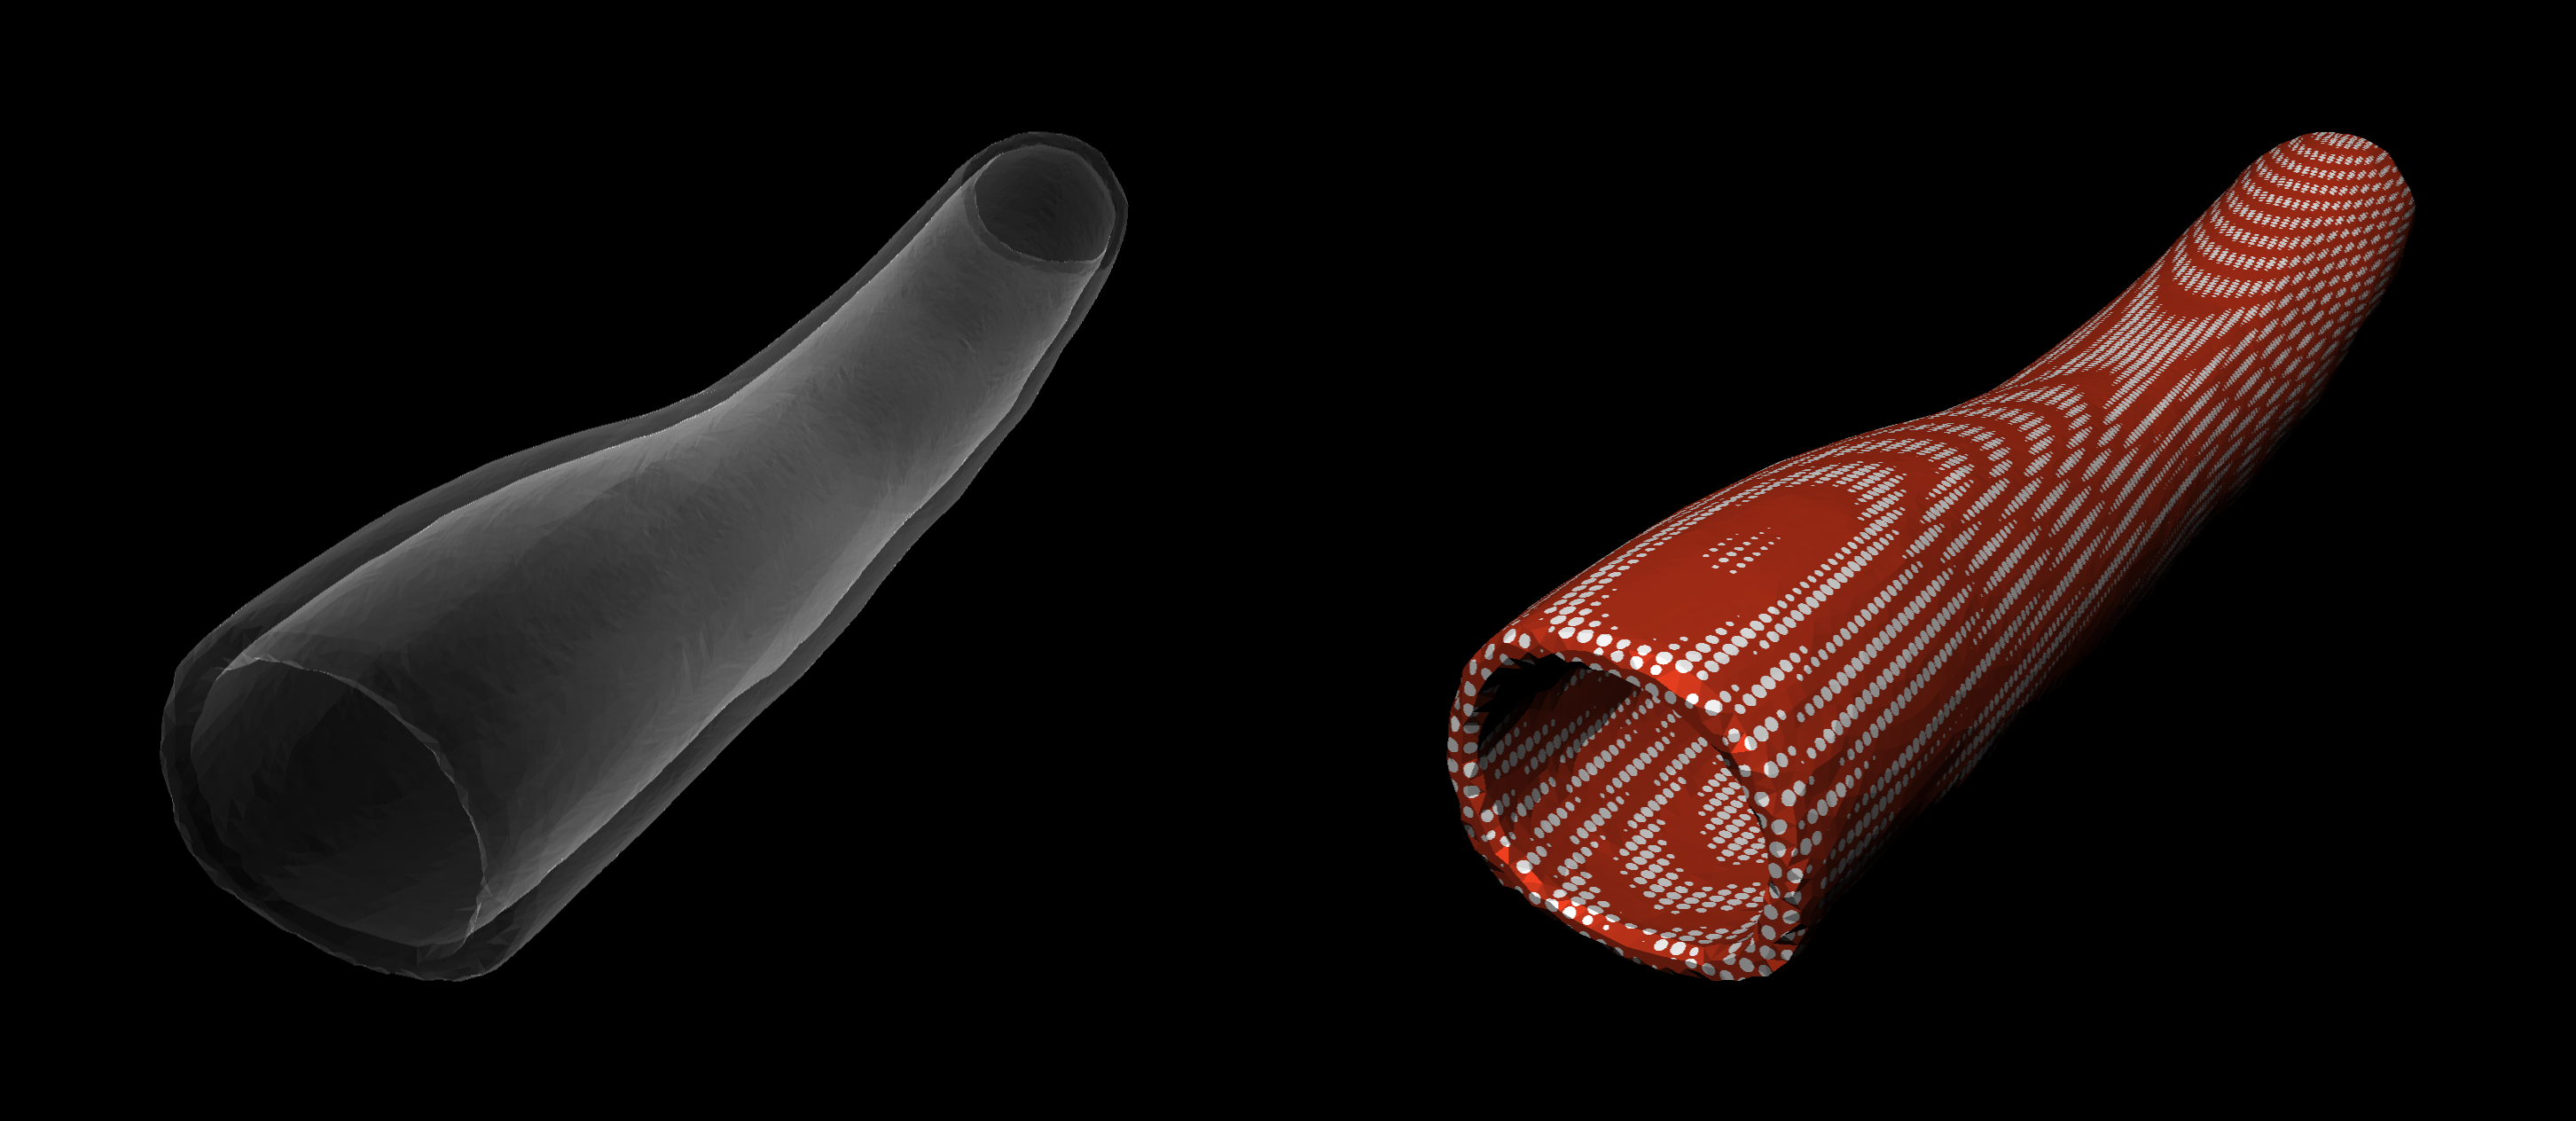
\includegraphics[width=\linewidth,frame]{models/urethra}
  \caption{Detailed volumetric model of a (hollow) urethra}\label{fig:urethra}
\end{figure}

\begin{figure}
  \centering%
  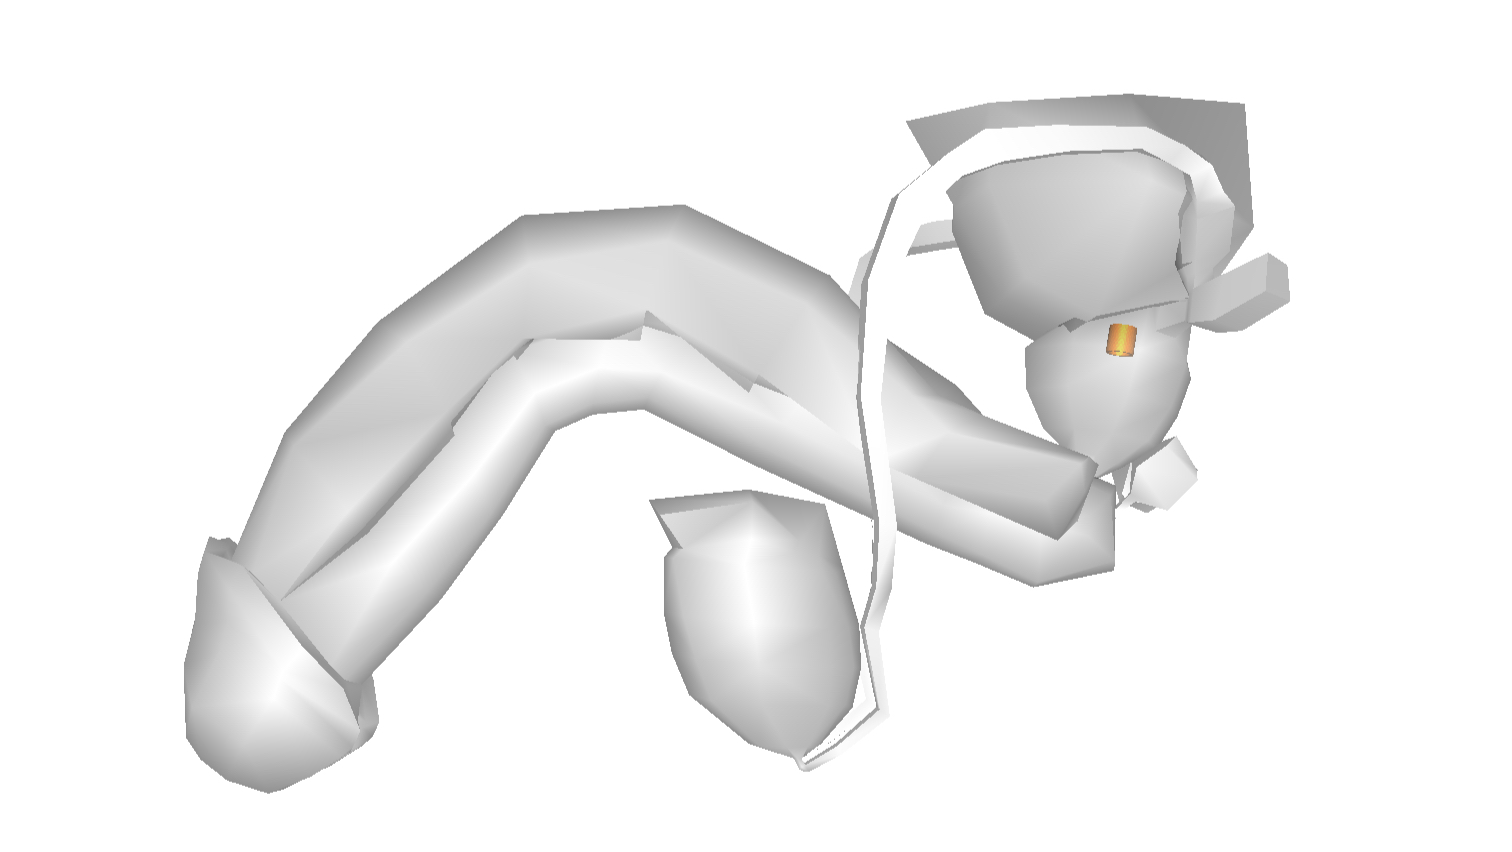
\includegraphics[width=\linewidth,frame]{models/overlay}
  \caption{Male reproductive system overlaid on top of a portion of interest of the urethra model. This display is helpful in navigating the initial scene and reorienting during the procedure}\label{fig:overlay}
\end{figure}

\subsection{Generation of Volumetric Models}\label{ssec:generation_volume}

In the previous task, we generated the triangular surface meshes for organs in the pelvic region by delineating \acr{mri} images. The triangular meshes representing tissue surfaces were further processed to generate two types of tissue models:
\begin{enumerate}
  \item Tissues structures solid from inside that are generated using a constrained Delaunay tetrahedralization algorithm \cite{tetwild} in form of volumetric tetrahedral mesh, \eg prostate, and
  \item Tissues structures hollow from inside that are generated using a constrained Delaunay tetrahedralization algorithm \cite{tetwild} in form of volumetric tetrahedral mesh, \eg urethra.
\end{enumerate}

MAPPING surfaces to tetrahedra to keep texture coordinates.

Textures were overlaid on the surfaces as a final step to improve the realism.

\begin{figure}
  \centering%
  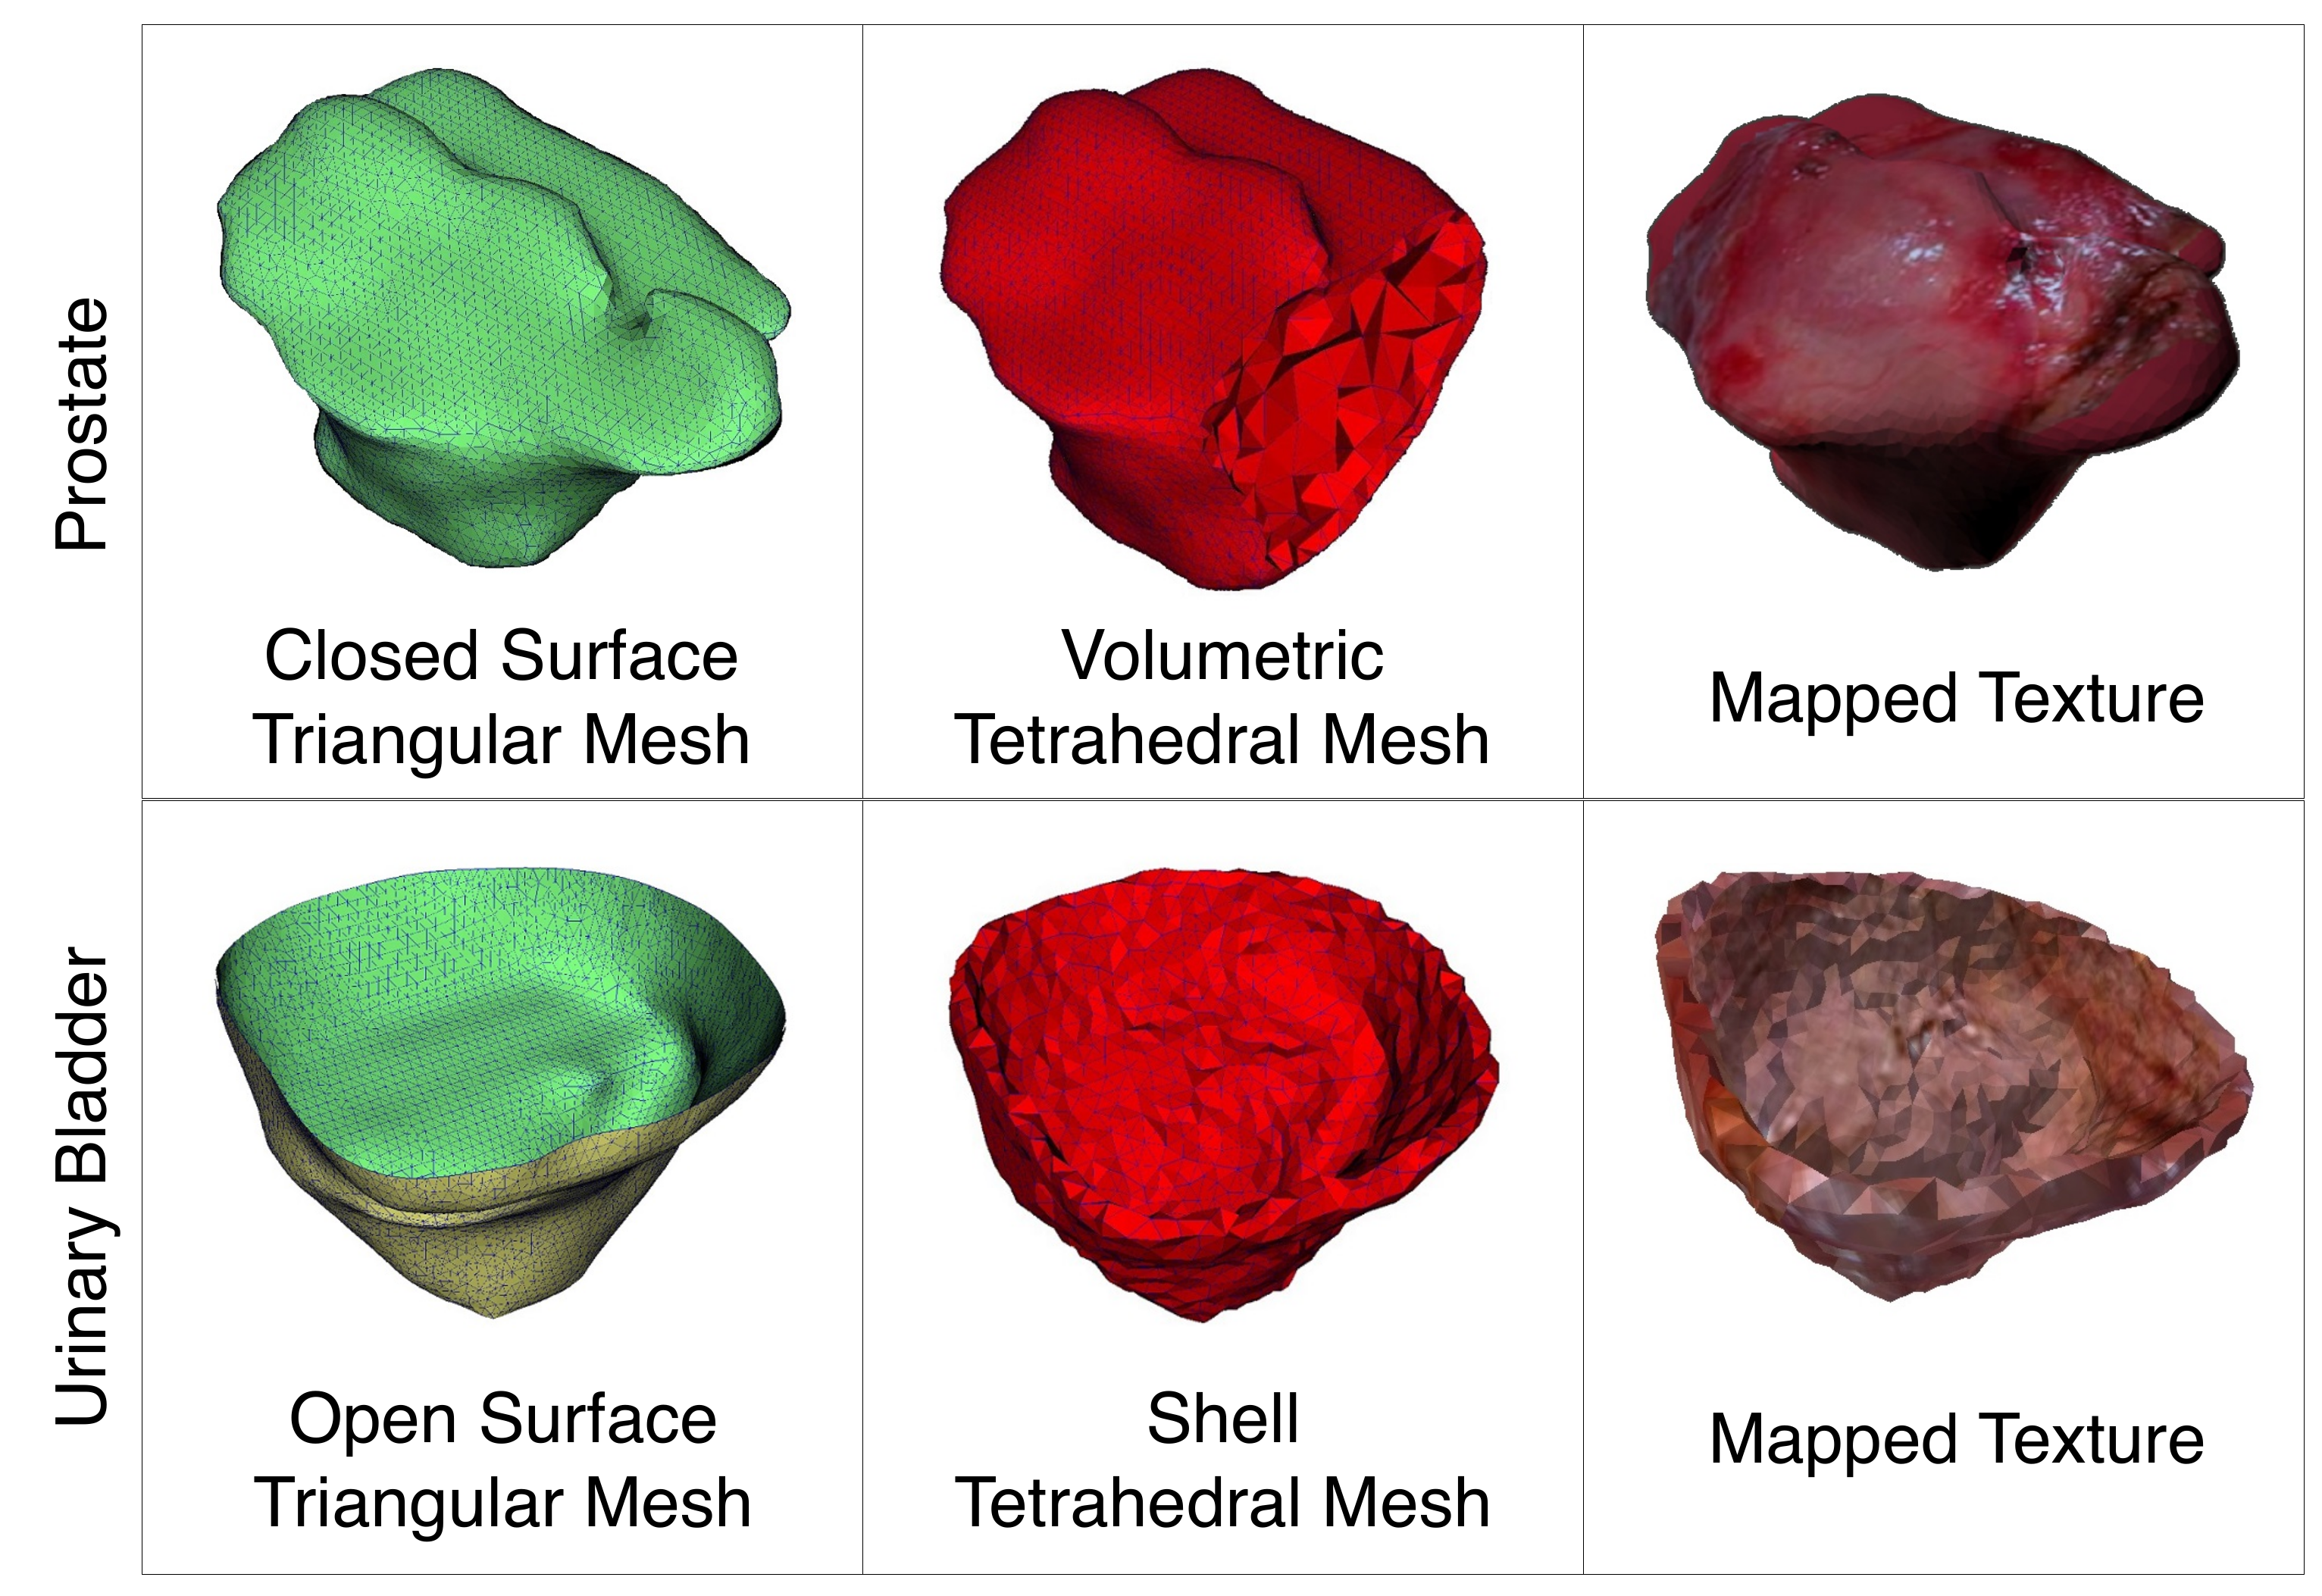
\includegraphics[width=0.75\linewidth]{models/pelvic_volumes}
  \caption{Volumetric meshes for prostate and bladder.}\label{fig:organ_prostate_bladder_generation}
\end{figure}

\subsubsection{Realistic Volumetric Models}
\autoref{fig:pbr_scene}, \autoref{fig:urethra_pbr_wireframe}, and \autoref{fig:urethra_pbr_foley}.

\begin{figure}
  \centering
  \includegraphics[width=1.0\textwidth,frame]{models/pbr_scene}
  \caption{The scene visualized using physically-based rendering}
  \label{fig:pbr_scene}
\end{figure}

\begin{figure}
  \centering
  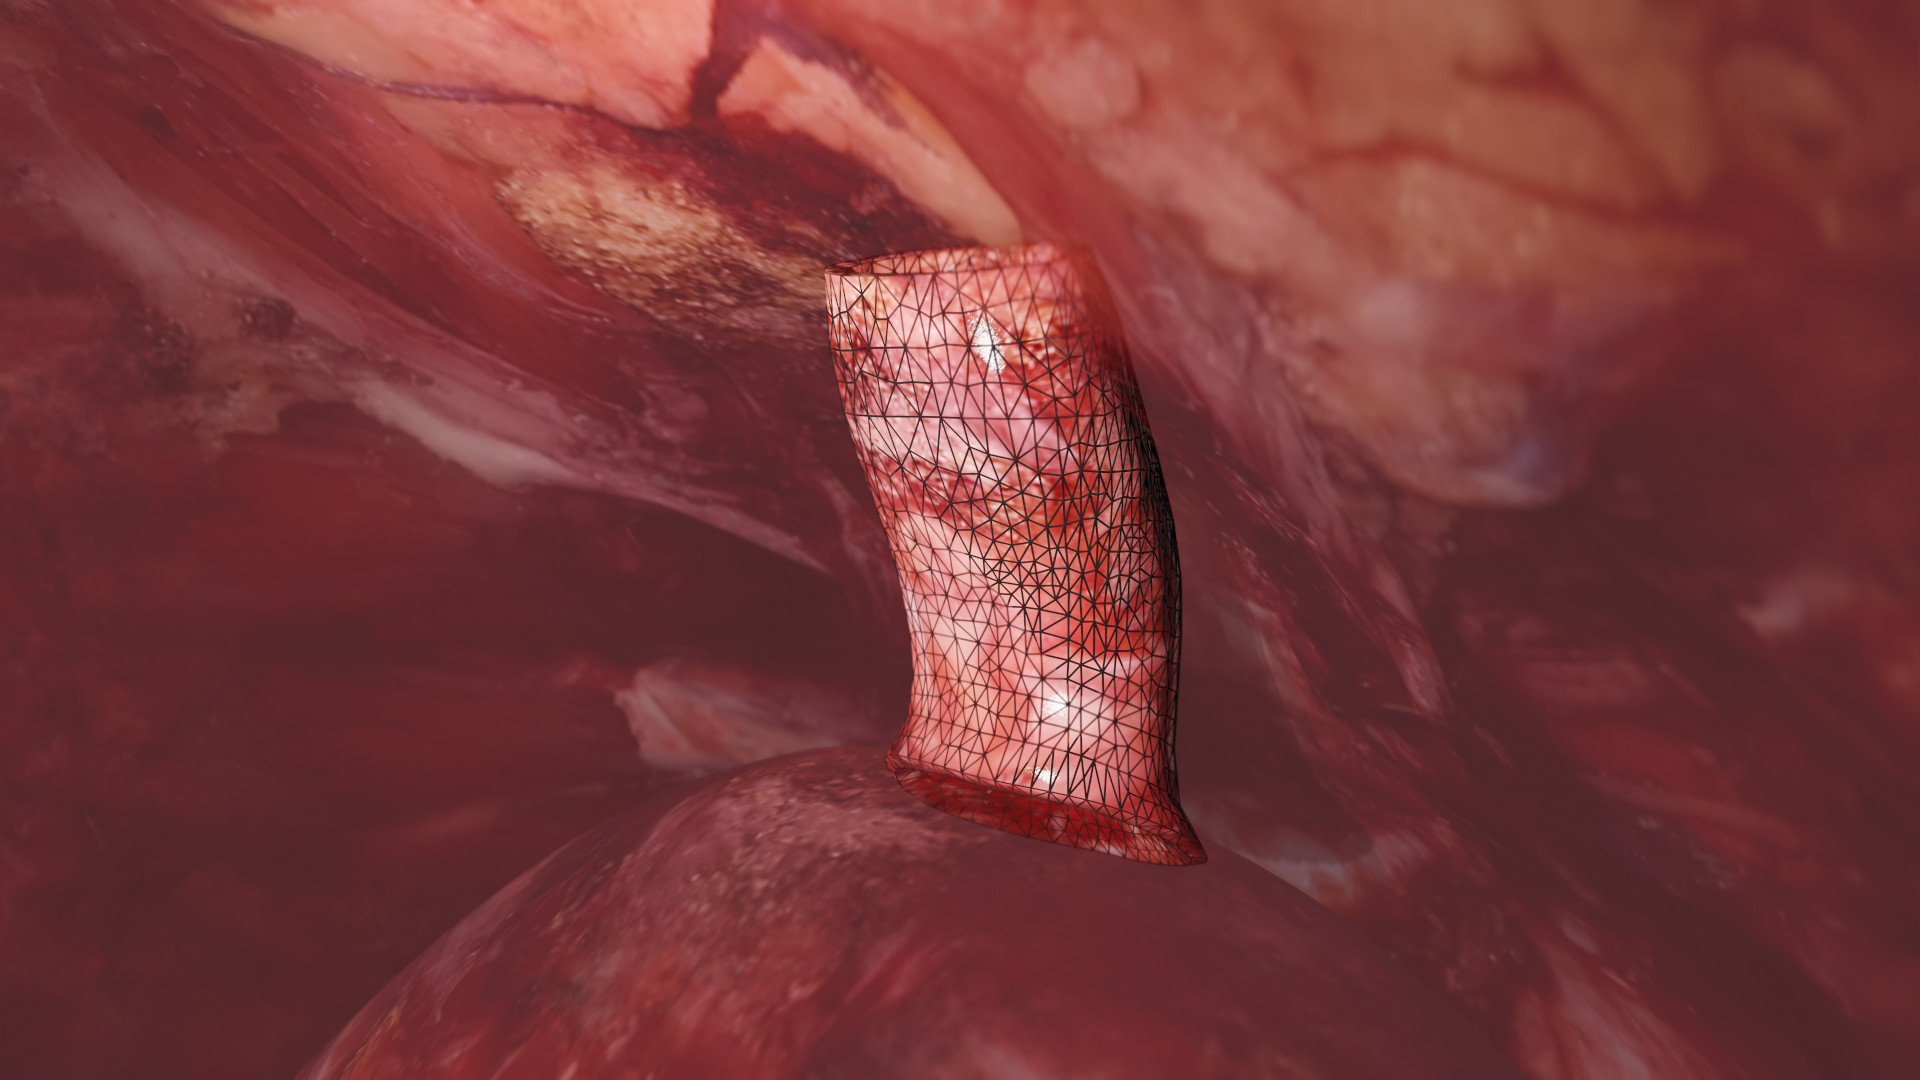
\includegraphics[width=1.0\textwidth,frame]{models/urethra_pbr_wireframe}
  \caption{The volumetric part of the urethra with translucent surrounding meshes}
  \label{fig:urethra_pbr_wireframe}
\end{figure}

\begin{figure}
  \centering
  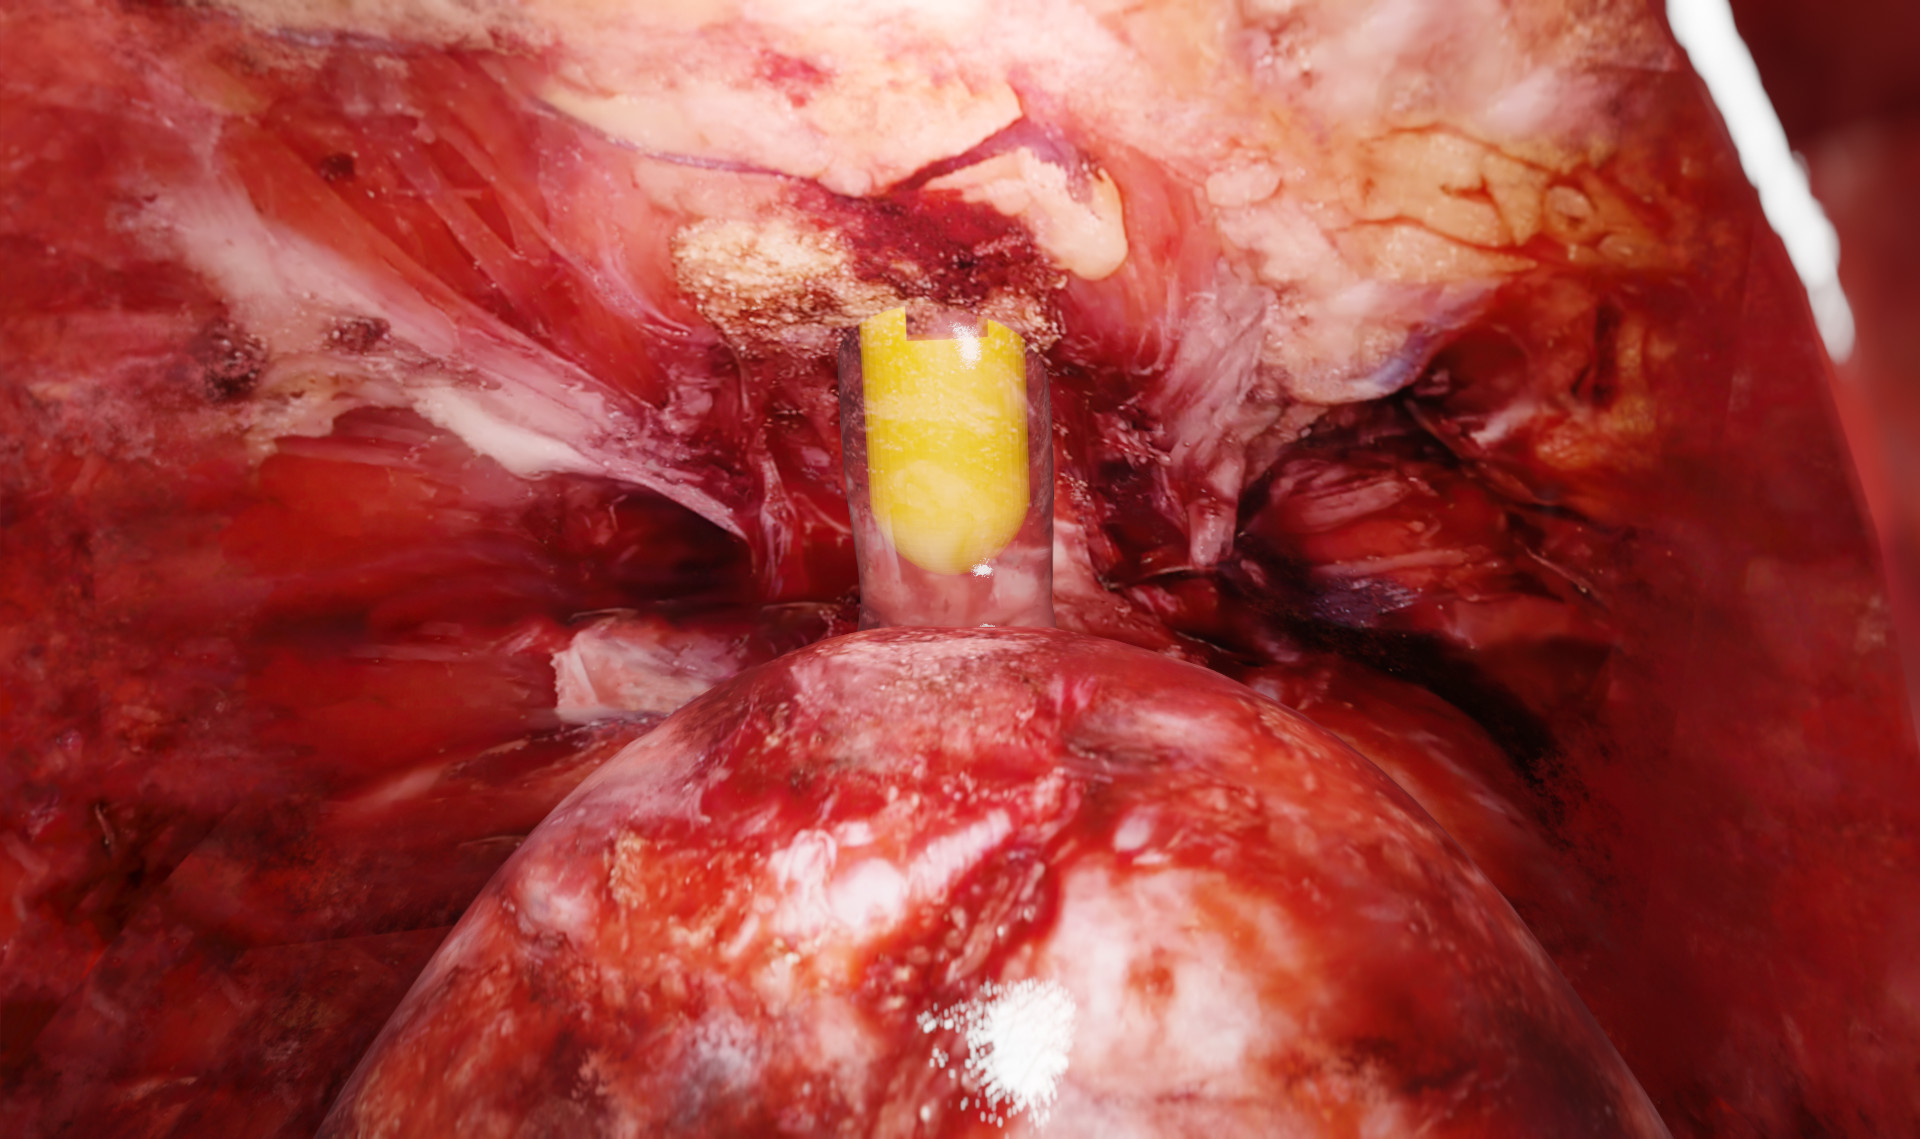
\includegraphics[width=1.0\textwidth,frame]{models/urethra_pbr_foley}
  \caption{A Foley catheter inserted midway through the (translucent) urethra}
  \label{fig:urethra_pbr_foley}
\end{figure}

\subsection{Texture Models}
We're currently extracting background scene and organ textures from stereoscopic recordings of robotic procedures performed at HMC. Our future plan is to extract volumetric textures as well, to render cuts more realistically.


\subsubsection{Textures from Stereoscopic Videos}\label{sssec:videos}
The textures were extracted from a stereoscopic recording of the procedure that is being simulated, and then pasted on top of the surface models that were generated in the previous step. The end result can be seen below.

\begin{figure}
  \centering%
  \setlength{\fboxsep}{0pt}%
  \setlength{\fboxrule}{0.1pt}%
  \fbox{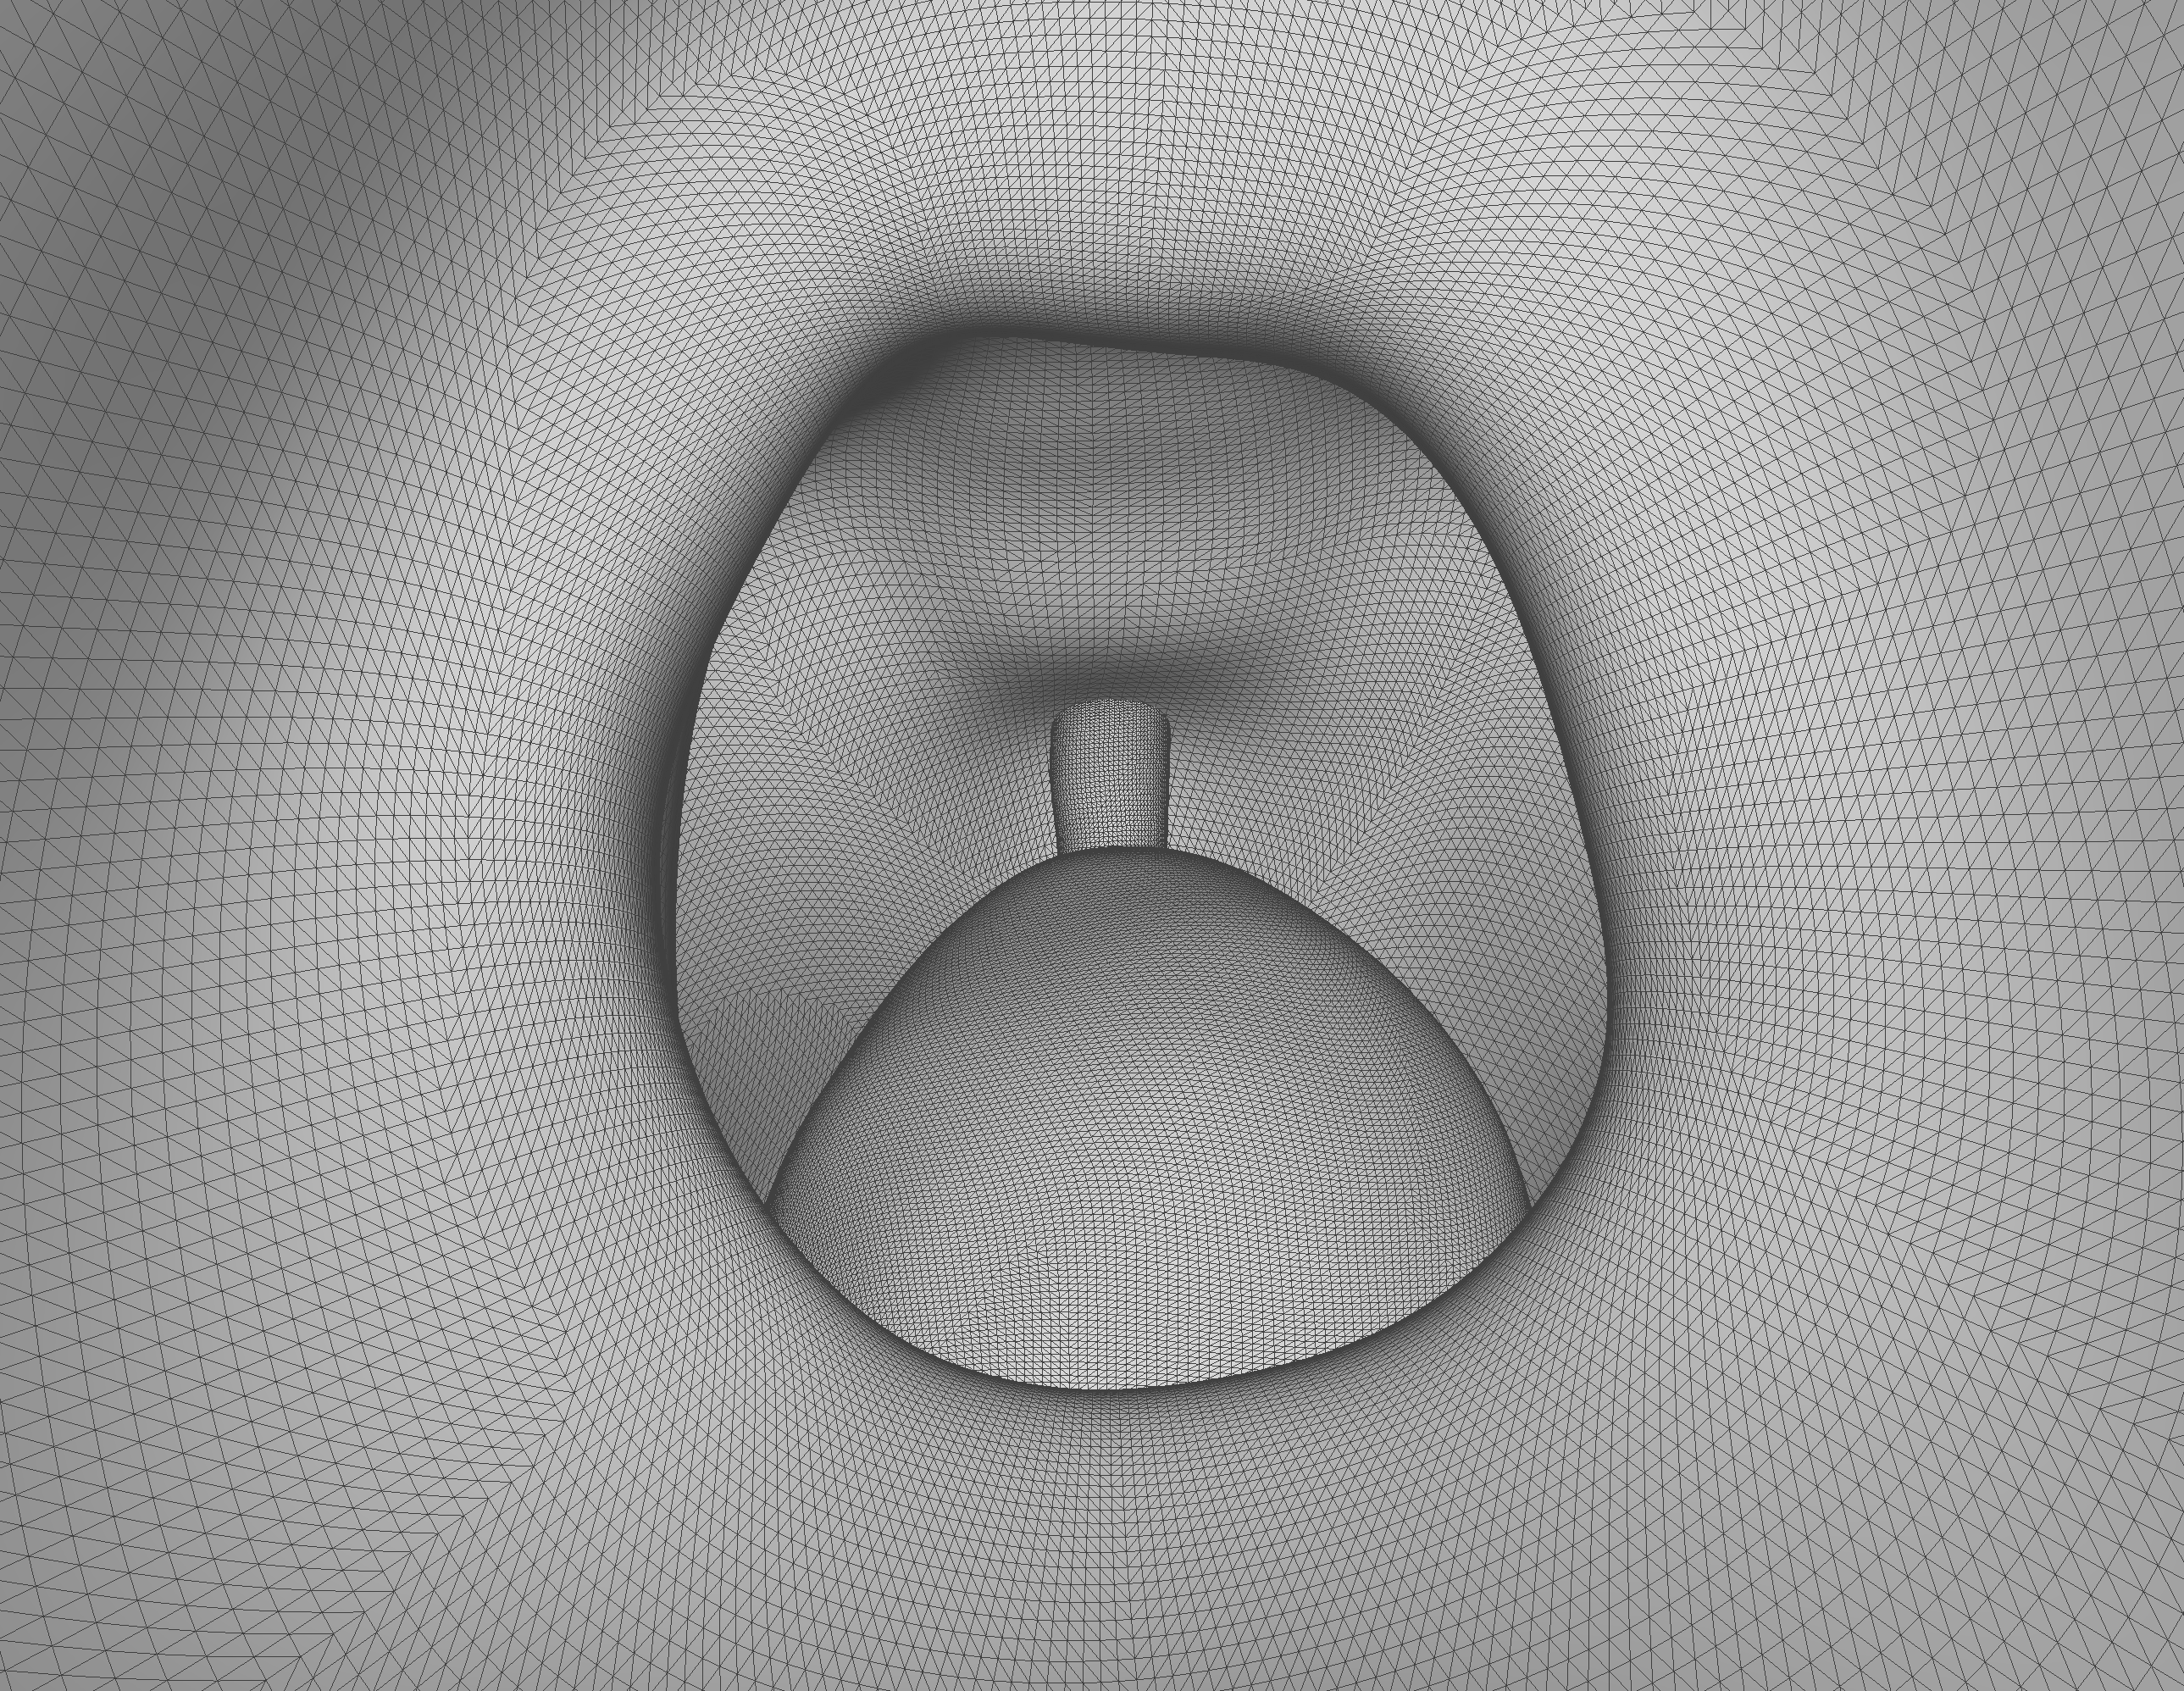
\includegraphics[width=0.48\linewidth]{models/edges}}
  \hfill%
  \fbox{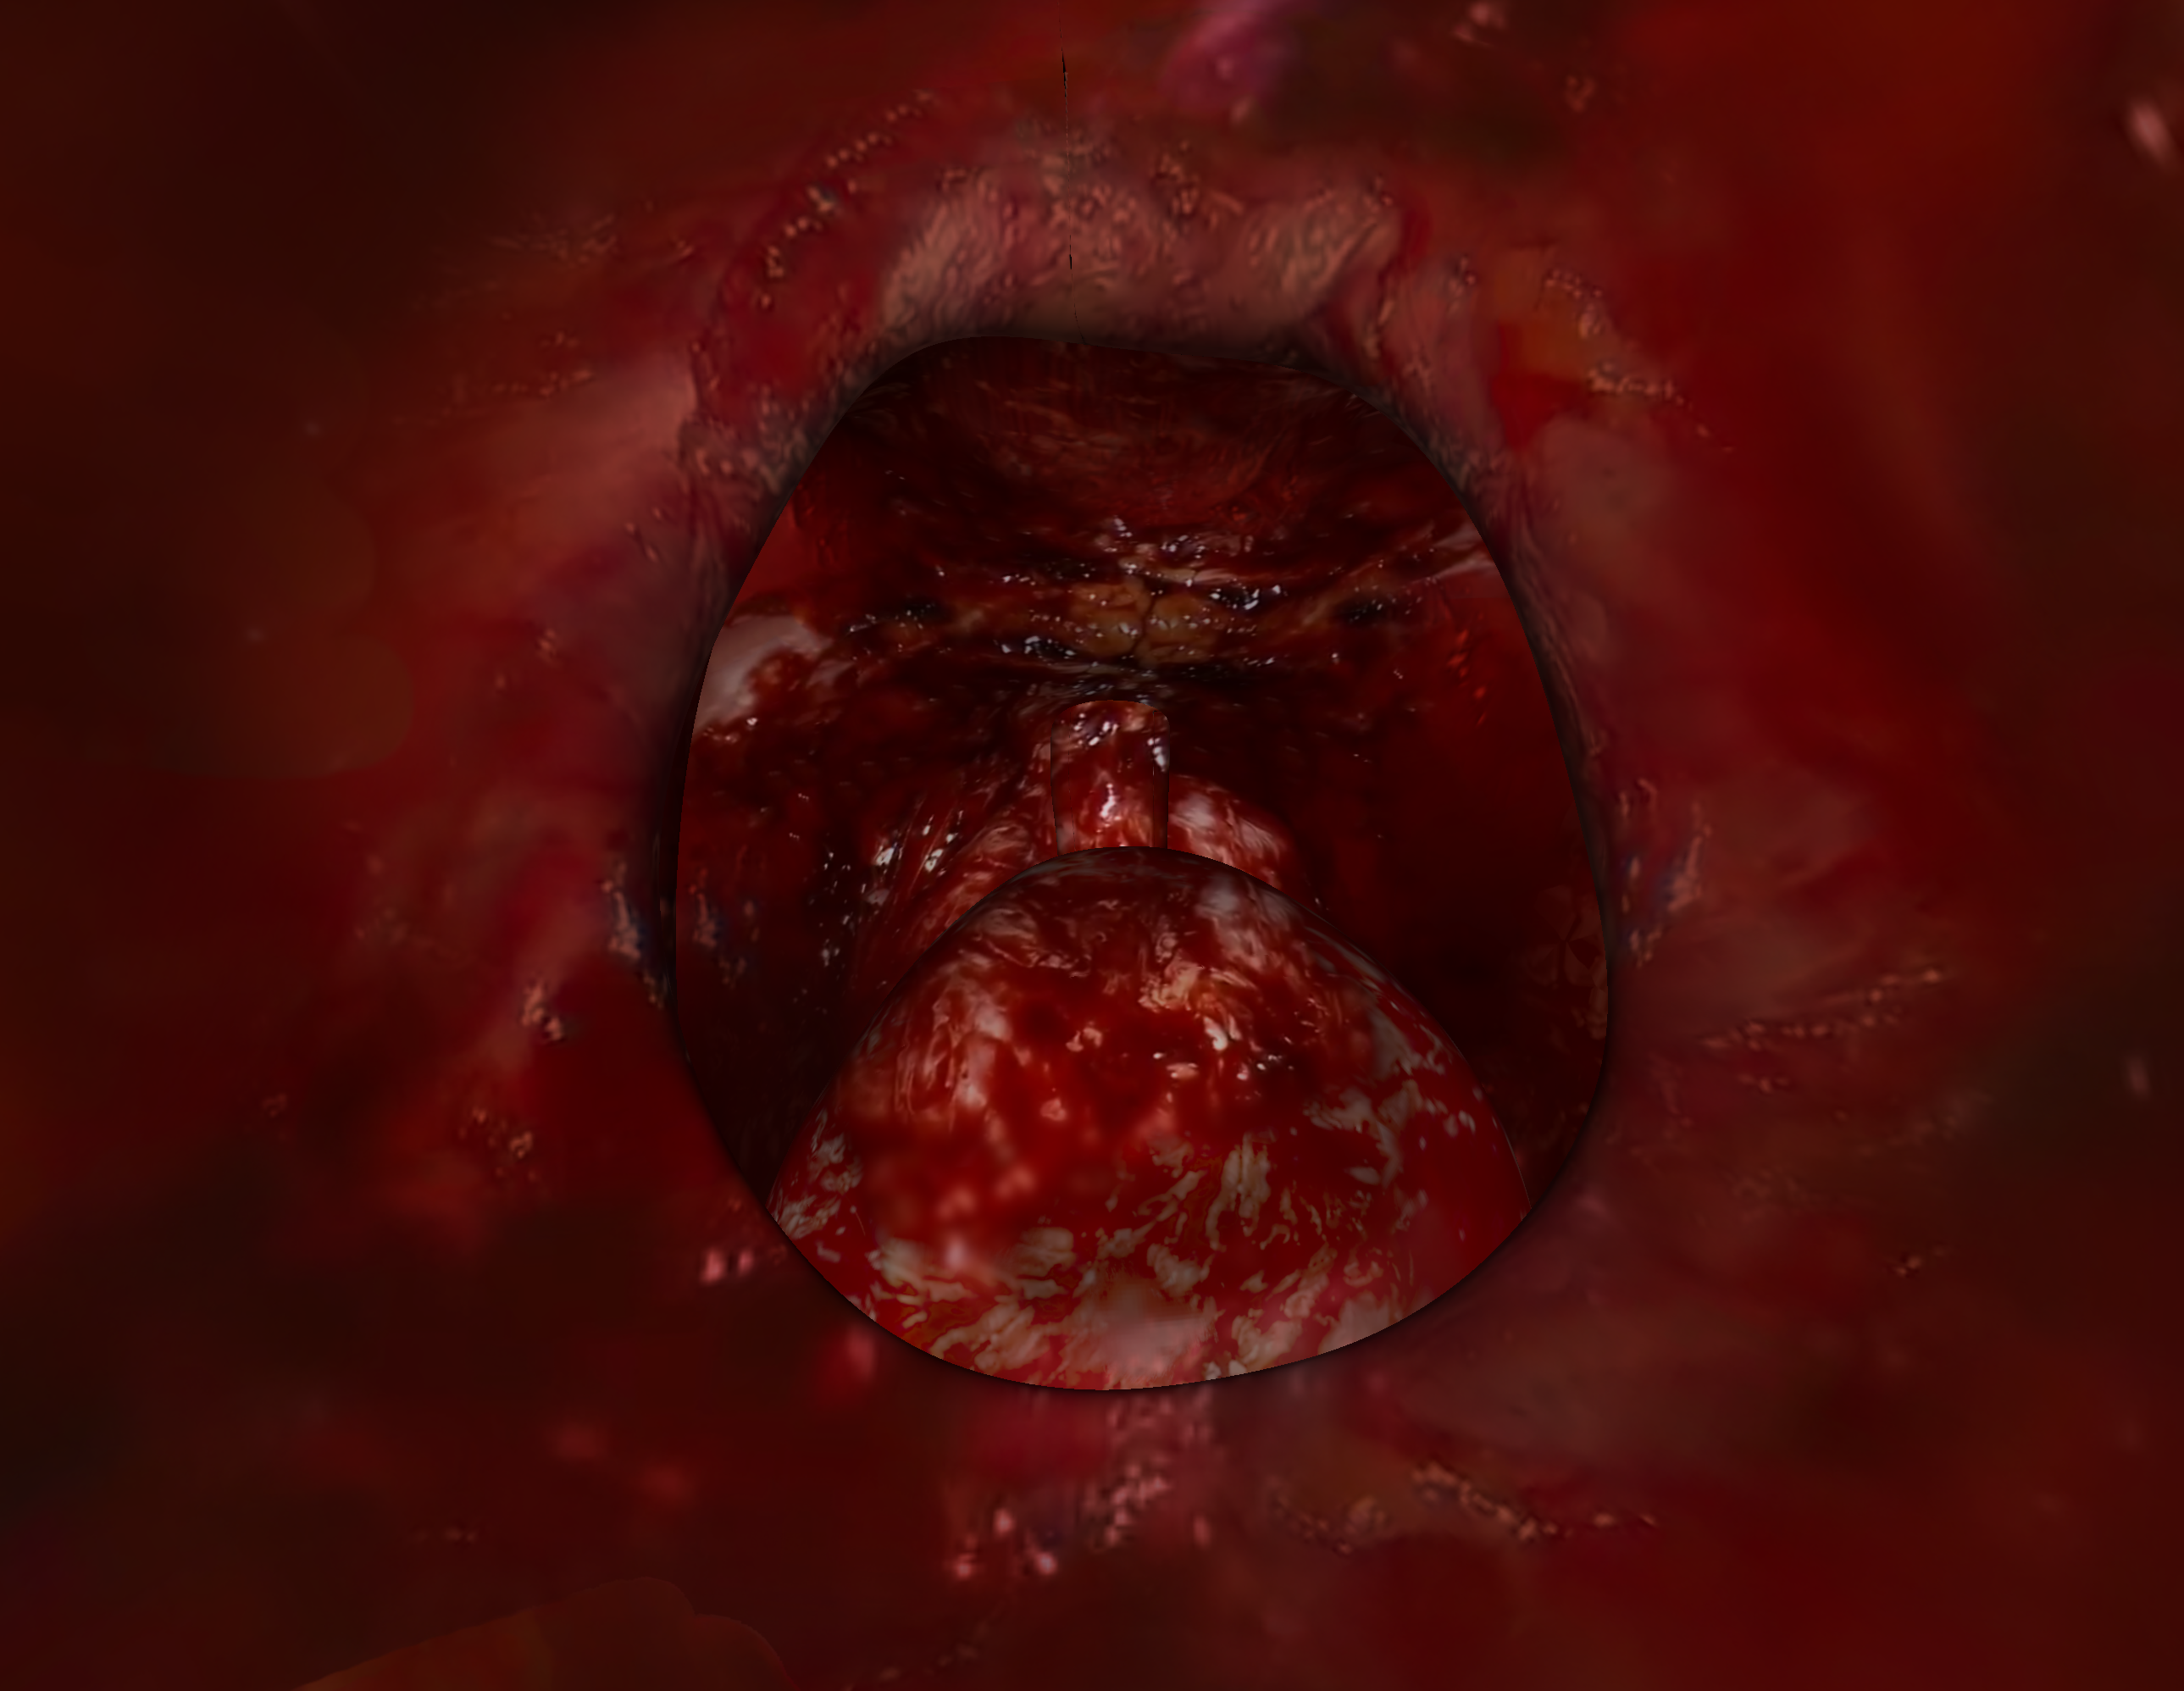
\includegraphics[width=0.48\linewidth]{models/textures}}
  \caption{---}\label{fig:texture_videos}
\end{figure}

\subsubsection{Procedural Textures}\label{sssec:procedural}
To produce seamless and realistic textures in the simulation, we opted to go for procedurally generated textures. Procedural textures are textures created from a user defined procedure instead of using predefined or existing image textures. This provides flexibility in customizing textures, not being limited by source image resolution and to generate textures for different meshes. Blender, a free and open source 3D creation suite supports creating procedural materials using visual programming. The generated textures can then be baked to static images in the required format for rendering later in OpenGL. By using procedural textures instead of textures from real images, we can reduce the time needed in preparing a model.

UV unwrapping a 3D model to a real image of the model to render the texture avoiding seams can be difficult and time consuming. Textures generated from the procedural materials account for the unwrapping, therefore less time can be spent on adjusting the UV coordinates. Moreover, procedural materials can be easily transferred onto other objects as the textures are generated based on the UV unwrapping that would be done beforehand.

\subsubsection{Real-time Rendering}
Blender comes packaged with the option to real-time render the scene which helps in previewing the generated procedural textures, speeding up the cycle of going back and forth between modifying the procedural material and seeing the result.

\begin{figure}
  \centering%
  \setlength{\fboxsep}{0pt}%
  \setlength{\fboxrule}{0.1pt}%
  \fbox{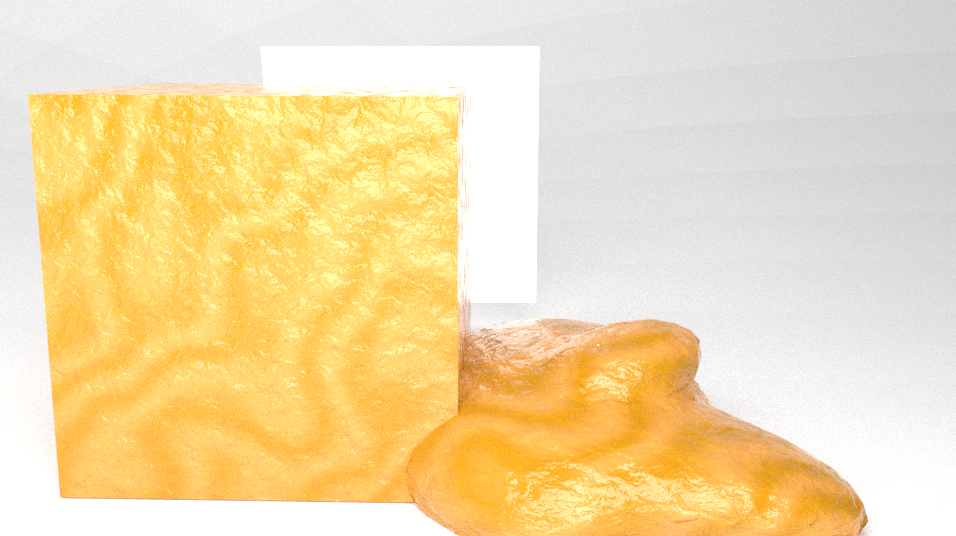
\includegraphics[width=\linewidth]{models/fat}}\\[2ex]
  \fbox{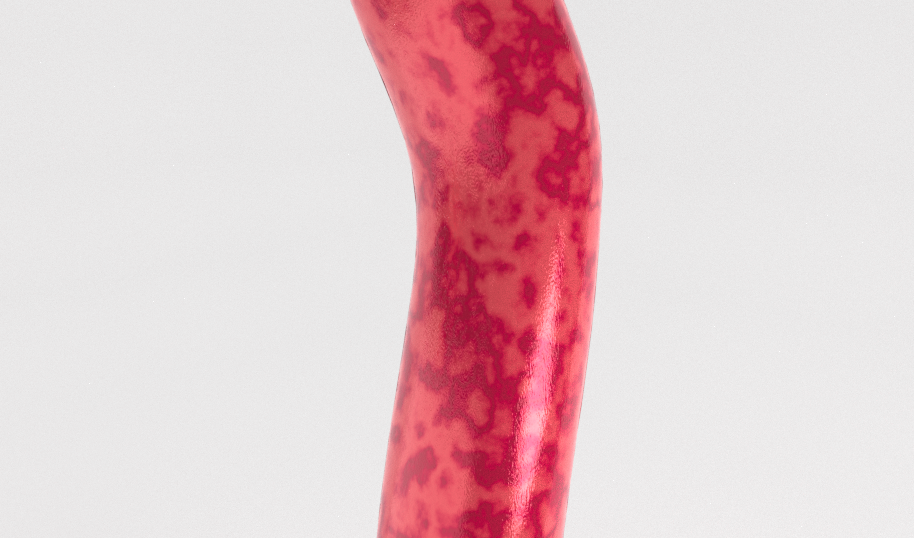
\includegraphics[width=\linewidth]{models/tissue}}
  \caption{Node editor in Blender.}\label{fig:procedural_textures}
\end{figure}

\subsubsection{Node Editor}
Node editor in blender provides a visual way to program the procedural material. The node editor comes with nodes such as different computer generated noise, image mixing, shaders, vector math nodes each with different customizability fields for achieving desired final result. Pairing this up with real-time rendered view leads to an efficient workflow for customizing and creating required materials. A snapshot is included below.

\begin{figure}
  \centering%
  \setlength{\fboxsep}{0pt}%
  \setlength{\fboxrule}{0.1pt}%
  \fbox{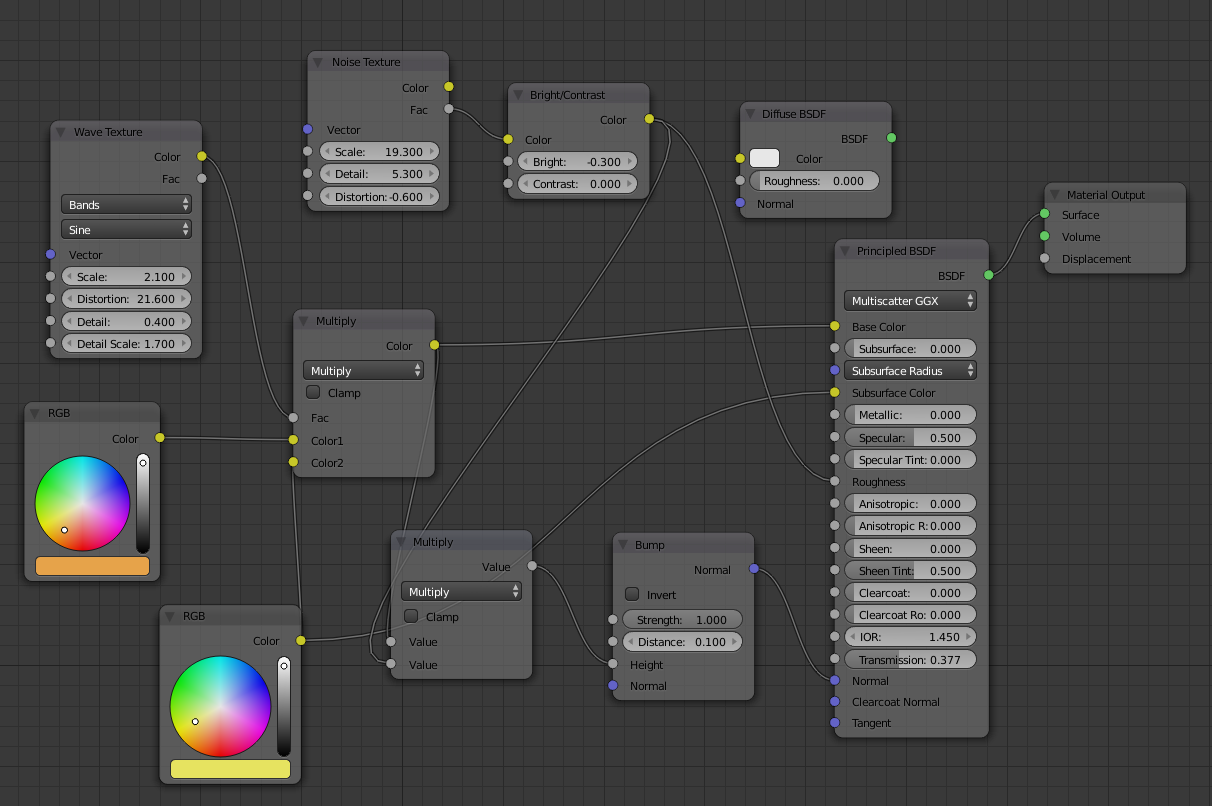
\includegraphics[width=\linewidth,frame]{models/blender}}
  \caption{Node editor in Blender.}\label{fig:blender}
\end{figure}

\subsubsection{Model Import}
The models used in our prototypes are volumetric models with tetrahedral structures stored using an OpenVolumeMesh data structure that can handle arbitrary polytopal meshes. Blender is used for surface meshes and is not meant for volumetric meshes. The goal was to import the volumetric mesh, then generate required textures and to export face to UV coordinates mapping for the mesh. However, converting a volumetric mesh to a surface mesh would cause loss of the faces that forms tetrahedrons except for the surface faces, and that could imply loss of vertices.

Unfortunately, it was hard to find methods to convert an OVM mesh to a surface mesh that could be read by blender. Since both VTK and OVM of a mesh had exact vertex to vertex mapping, importing either of them would be fine. We were able to device of two ways to convert a VTK structure into a surface mesh:

\begin{enumerate}[1.]
  \item Import VTK into ParaView and export as supported surface mesh formats, or
  \item Use the VTK Python library, along with VTKBlender library for importing the VTK directly into blender.
\end{enumerate}

Trying out the first method lead to loss of vertices therefore defeating the possibility of exporting UV coordinates. For the second option, the VTK library provided two ways to convert a VTK structure into a surface mesh. The first method was to use surface filter provided by the VTK library, which produced the surface mesh accurately but unused vertices were removed. The second method was to use a geometry filter provided by the same. The latter provided a surface mesh accurately as well, but with all the vertices intact. This meant we could obtain a relationship between the original VTK or OVM and the surface mesh in blender, hence allowing us to successfully map boundary faces of the volumetric mesh to UV coordinates.

\subsubsection{Texture Export}
Once UV unwrapping was done to the imported object and procedural material applied, the process of generating textures was straight forward. Blender provides a way to bake textures which gets the applied material and the UV unwrapping, and generates an image texture based on them.

The surface mesh generated by VTK and VTKBlender library retained all vertices but only kept the surface faces. Due to this, faces between the volumetric mesh and the surface mesh do not have a one to one mapping. However, we can determine the face in the surface mesh that corresponds the face in the volumetric mesh from the vertices for each face.

The surface mesh along with UV coordinates were exported in OBJ format which contains mapping of vertices for each face, and texture coordinates of each vertex for each face. The OVM structure contains face to half-edge mapping, and half-edges have information about two vertices (from- and to- vertex). We managed to create a Python script which maps OBJ faces to OVM faces and then output a file representing face id in OVM and texture coordinates for each unique vertex. The figure below shows the relationship of an OVM face to its corresponding UV coordinates.

We're currently working on generating solid textures that would allow us to render the newly introduced faces, following a cut, properly and more realistically.

\subsubsection{Solid Textures with Random Noise}
The surfaces of the volumetric meshes were textured appropriately by UV unwrapping an identical surface mesh and then mapping UV coordinates to the corresponding surface triangles in the volumetric mesh.

Two types of surface triangles are generated when a user performs a cut on the volumetric mesh. One is parallel to the cut surface and newly introducted, and the other results from subdividing previous surface triangles. In the latter case, we use barycentric coordinates to interpolate the texture coordinates for the resulting triangle from which it was subdivided.

However, for the newly introduced surface triangles that are parallel to the cut surface, we had to follow a different approach. Since the user can cut anywhere on the volumetric mesh, we would need volumetric textures to be super imposed on the newly generated triangles in 3D space.

For the visual look of the cut surface, we chose to use a 3D perlin noise function with tweaked parameters to visualize the cut. We looked into two approaches for volumetric textures. One approach was to generate an $n \times n \times n$ texture using a 3D noise function and then pass it as a 3D texture with OpenGL's \texttt{TEXTURE3D} interface. The other approach was to dynamically generate them within the shader using the 3D noise function. Generating a high resolution volumetric texture that engulfs the whole mesh is time consuming and results in a large memory footprint. Generating a cube texture of dimensions $1000 \times 1000 \times 1000$ would be equivalent of a thousand $1000 \times 1000$ 2D images with the noise computed for each pixel. The second approach seemed to be the better option as the 3D noise function is used only for the pixels within the newly generated triangles and resulted in better performance.

Regardless of the approach, to have continuous textures between cuts, the UVW coordinates (3D coordinates for 3D textures) must be continuous and consistent. By passing the actual XYZ positions of the vertices as UVW coordinates we can render continuous textures between cut surface triangles. However, during user interactions, the texture would change as the mesh deforms because the positions and UVW are the same. To prevent this from happening we use the initial (rest state) coordinates of the vertices in the mesh as UVW coordinates. This initial rest state mesh vertex positions can be considered as UVW mapping of the mesh. The remaining aspect to cover is for the newly generated vertices. These are interpolated using the nearest initial vertices.

\begin{figure}
  \centering
  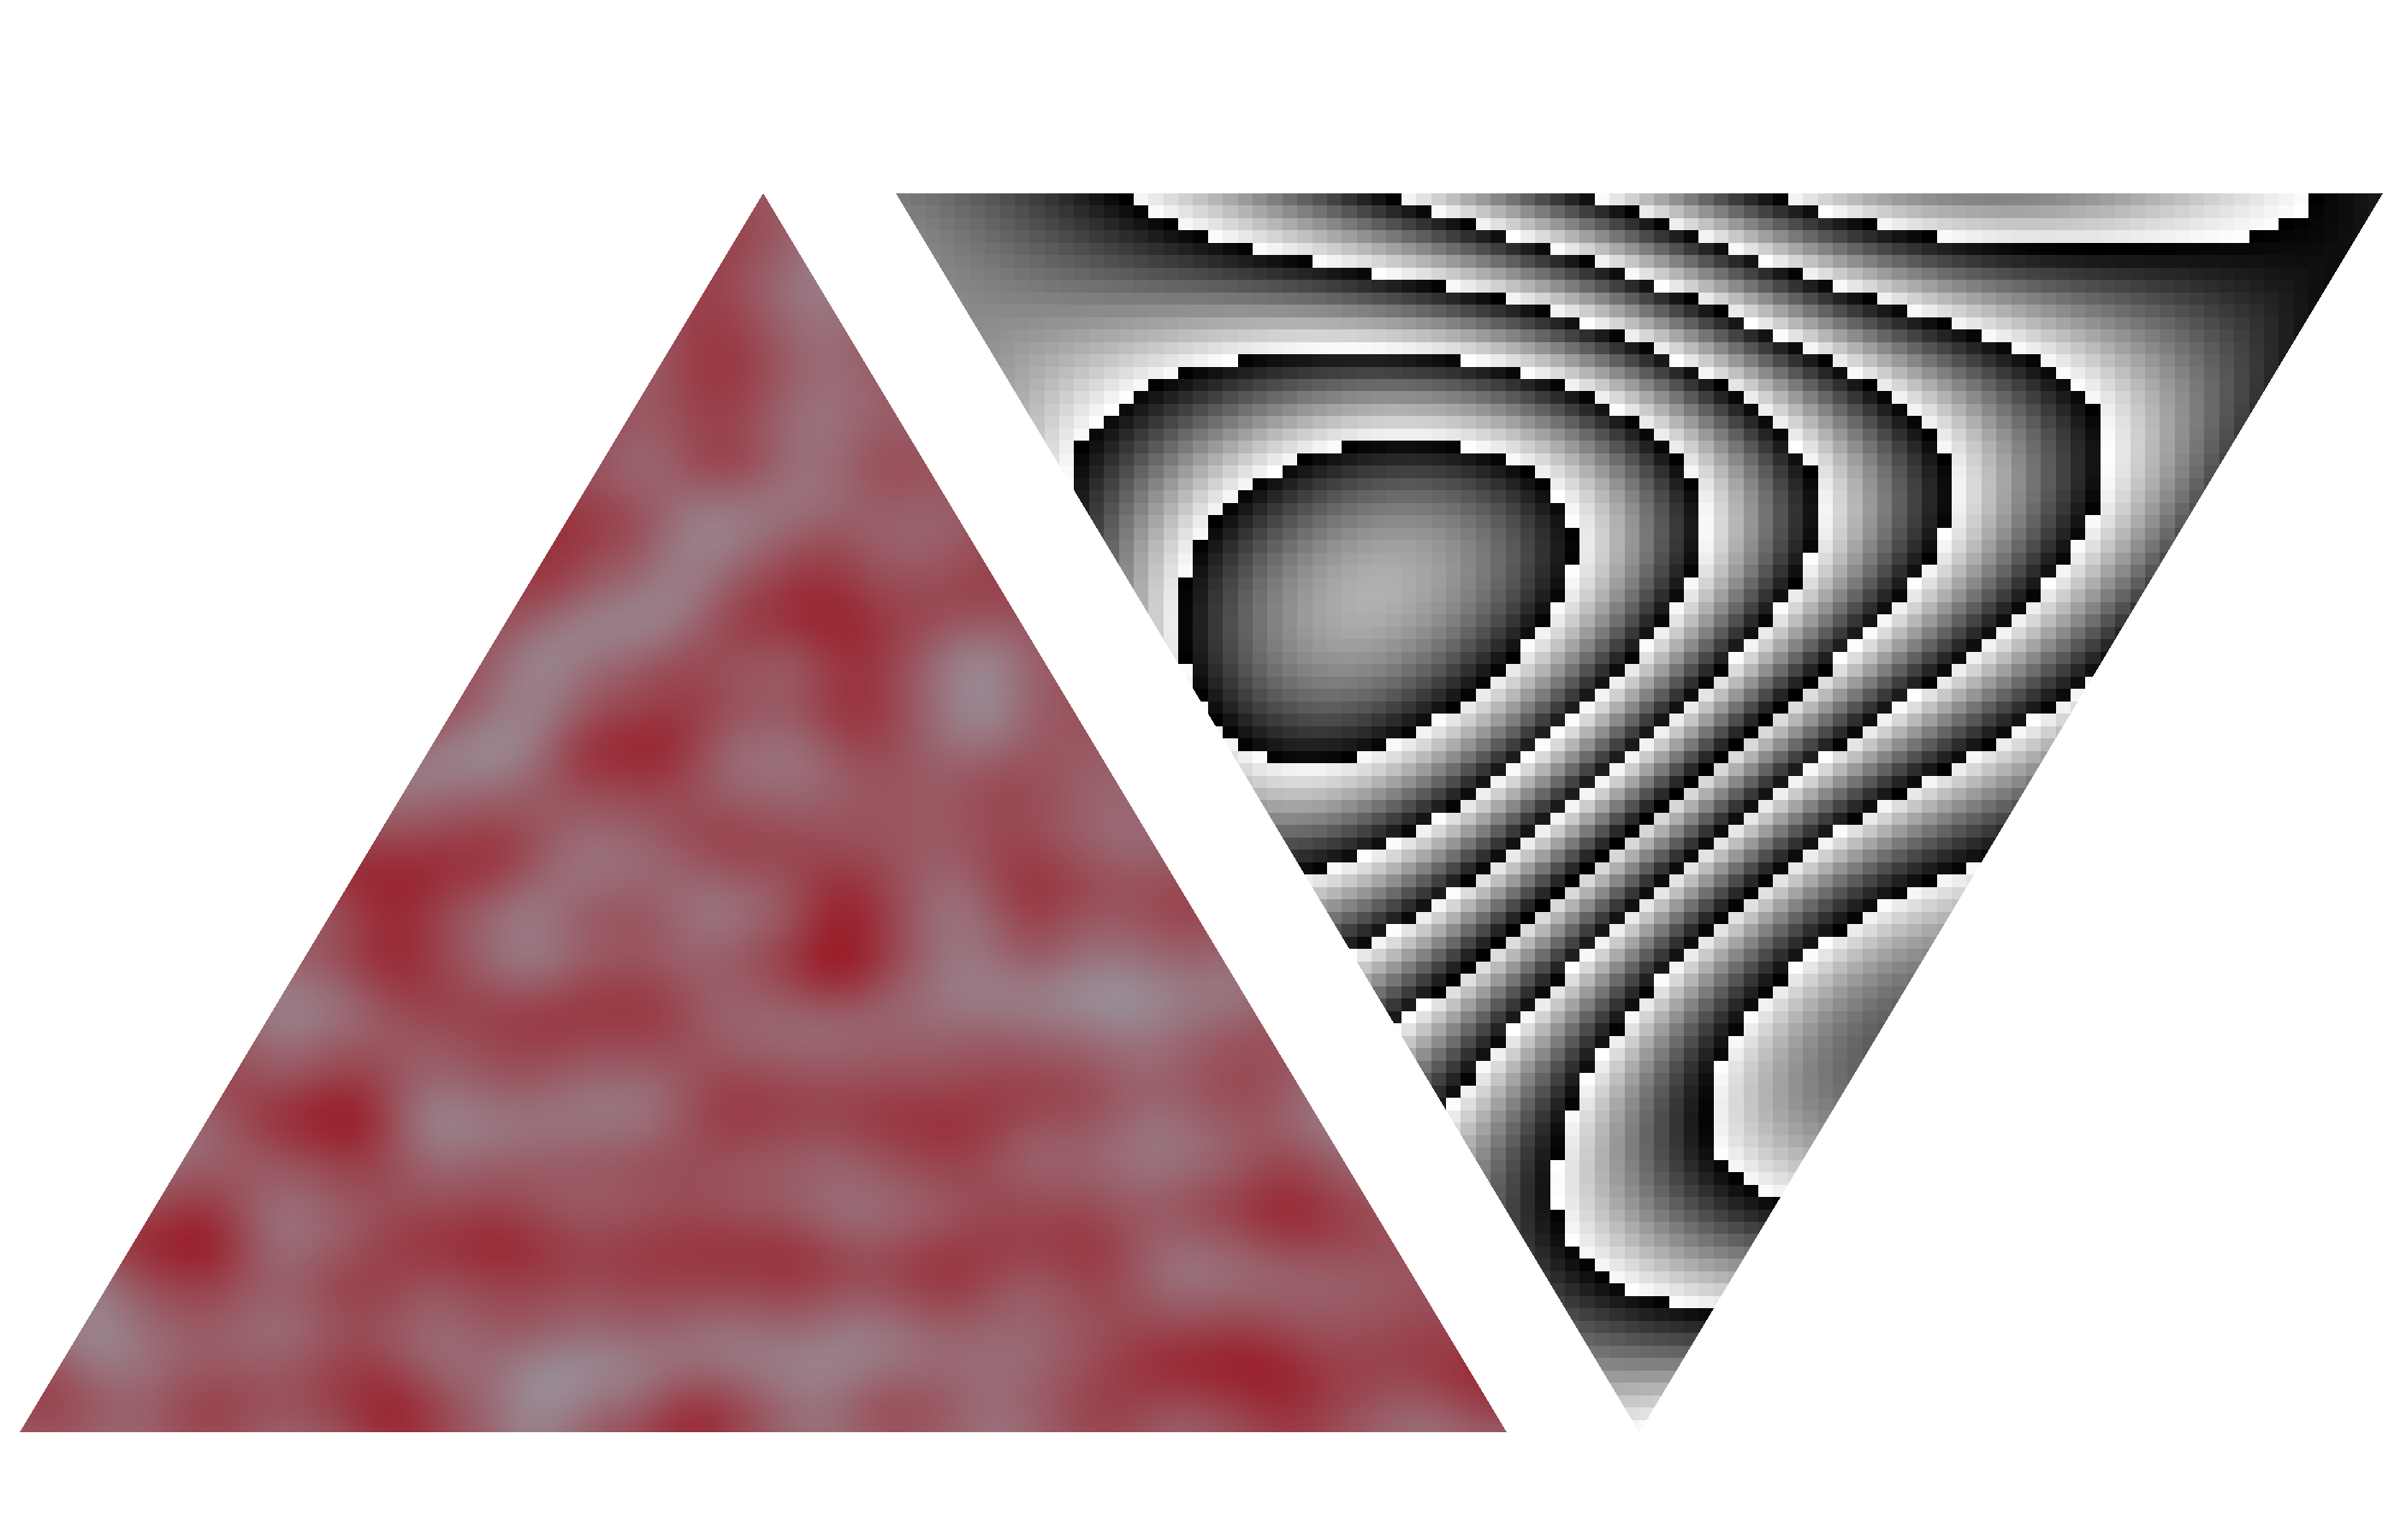
\includegraphics[width=0.6\textwidth]{models/solid_textures}
  \caption{Shader-based noise texture on the left and precomputed noise texture on the right}\label{fig:solid_textures}
 \end{figure}

\subsection{Material Models}
We've created basic isotropic material models for the urethra and bladder and are iteratively calibrating their parameters using feedback from the experts that are testing out our prototype. Once they're finalized, we'll encode them into our mesh models.

Volumetric models were generated using the TetWild library, which produces meshes that are suitable for \acr{fem} simulations, by using the surface models as input. The output tetrahedral meshes are rendered below.

\begin{figure}
  \centering%
  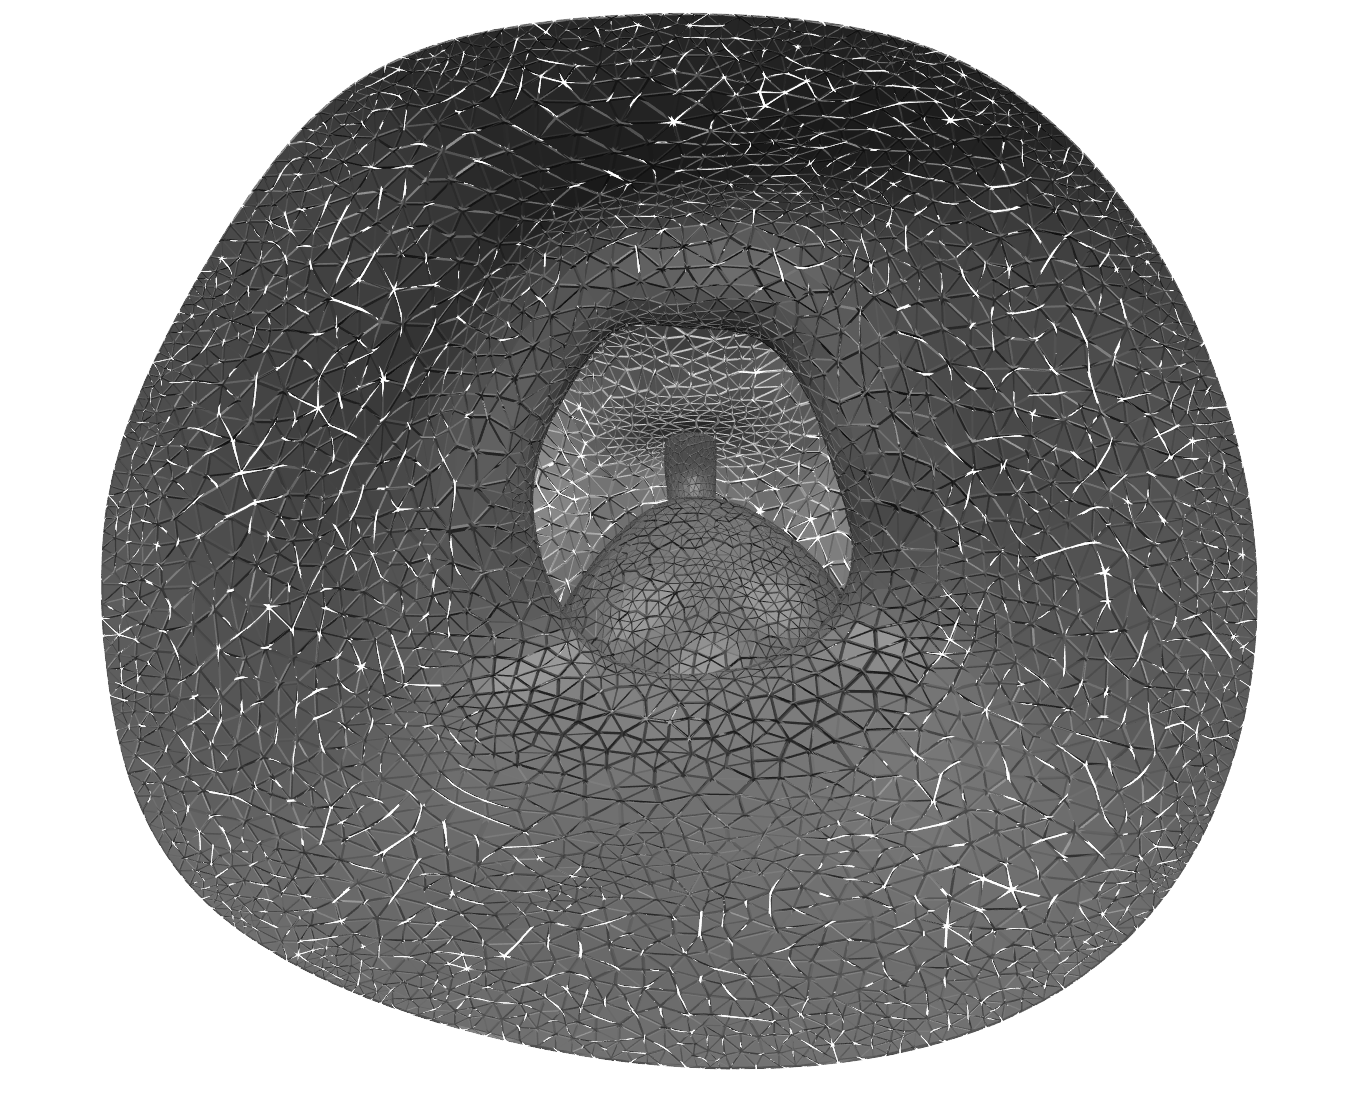
\includegraphics[width=0.8\linewidth]{models/tets}
  \caption{---}\label{fig:tetra_meshes}
\end{figure}

We're currently at the last step of tweaking the physical parameters to match with the surgeons' expectations.

\clearpage%
